\begin{frame}{Module Level DQ Checks}
    \begin{itemize}
        \item Some new variables were introduced in the 2024 data
        \begin{itemize}
            \item module\_eta0, module\_phi0
            \item which describes the first tracking module hit by the particle
        \end{itemize}
        \item Idea is to look at the track variables as a function of this
        \begin{itemize}
            \item Since, variables not present in 2023 data
            \item Eta0 and Phi0 are estimated using Track\_x0 and Track\_y0
        \end{itemize}
        % \item Unfortunately, 8 modules across 2 year = 16 Histograms 
        % \begin{itemize}
        %     \item Hard to visualize, so we do a module level comparison
        %     \item More detailed plots available in the backup/repo
        % \end{itemize}
        

    \end{itemize}
\end{frame}

\begin{frame}{Module Numbering Schematic }
    \begin{figure}
        \hspace{-1cm}
        \begin{tikzpicture}[scale=0.24]
            % \draw[step=1cm,gray!30,very thin] (-12,-12) grid (12,12);

            \draw[-,thick] (0,-12) -- (0,12);
            \draw[-,thick] (-12,-12) -- (-12,12);
            \draw[-,thick] (12,-12) -- (12,12);


            \draw[-, thick] (-12, -12) -- (12, -12);
            \draw[-, thick] (-12, -6) -- (12, -6);
            \draw[-, thick] (-12, 0) -- (12, 0);
            \draw[-, thick] (-12, 6) -- (12, 6);
            \draw[-, thick] (-12, 12) -- (12, 12);

            \node[rectangle, draw=none, minimum size=1pt] at ( -6 , 9 )  {Module 1};
            \node[rectangle, draw=none, minimum size=1pt] at ( -6 , 3 )  {Module 2};
            \node[rectangle, draw=none, minimum size=1pt] at ( -6 , -3 ) {Module 3};
            \node[rectangle, draw=none, minimum size=1pt] at ( -6 , -9 ) {Module 4};

            \node[rectangle, draw=none, minimum size=1pt] at ( 6 , -9 )  {Module 5};
            \node[rectangle, draw=none, minimum size=1pt] at ( 6 , -3 )  {Module 6};
            \node[rectangle, draw=none, minimum size=1pt] at ( 6 , 3 )   {Module 7};
            \node[rectangle, draw=none, minimum size=1pt] at ( 6 , 9 )   {Module 8};

            \draw[->, thick] (-13, -13) -- (-13, 13.5) node[above right] {$y$};
            \draw[->, thick] (-13, -13) -- (13, -13) node[right] {$x$};
            
            \draw[- , thick] (-13, -12) -- (-12.5, -12) node[left=0.1cm] {-120}; 
            \draw[- , thick] (-13,  -6) -- (-12.5,  -6) node[left=0.1cm] {-60}; 
            \draw[- , thick] (-13,   0) -- (-12.5,   0) node[left=0.1cm] {0}; 
            \draw[- , thick] (-13,   6) -- (-12.5,   6) node[left=0.1cm] {60}; 
            \draw[- , thick] (-13,  12) -- (-12.5,  12) node[left=0.1cm] {120}; 

            \draw[- , thick] (-12, -13) -- (-12, -12.5) node[below=0.1cm] {-120};
            \draw[- , thick] (0,   -13) -- (0,   -12.5) node[below=0.1cm] {0}; 
            \draw[- , thick] (12,  -13) -- (12,  -12.5) node[below=0.1cm] {12}; 

            \node at (-17, -9) {Phi = 0};
            \node at (-17, -3) {Phi = 1};
            \node at (-17, +3) {Phi = 2};
            \node at (-17, +9) {Phi = 3};

            \node at (-6, -14.7) {Eta = -1};
            \node at (+6, -14.7) {Eta = +1};

            % \node[rectangle, draw=none, minimum size=1pt] at ( -6 , 9 )  {Module 1};
        \end{tikzpicture}
        \caption{Module Boundaries Schematic. Numbering borrowed from Angela's Schematic}
    \end{figure}
\end{frame}

% \begin{frame}{Module Level Splitting}
%     \begin{columns}
%         \begin{column}{1.2\linewidth}
%             \begin{figure}
%                 \centering
%                 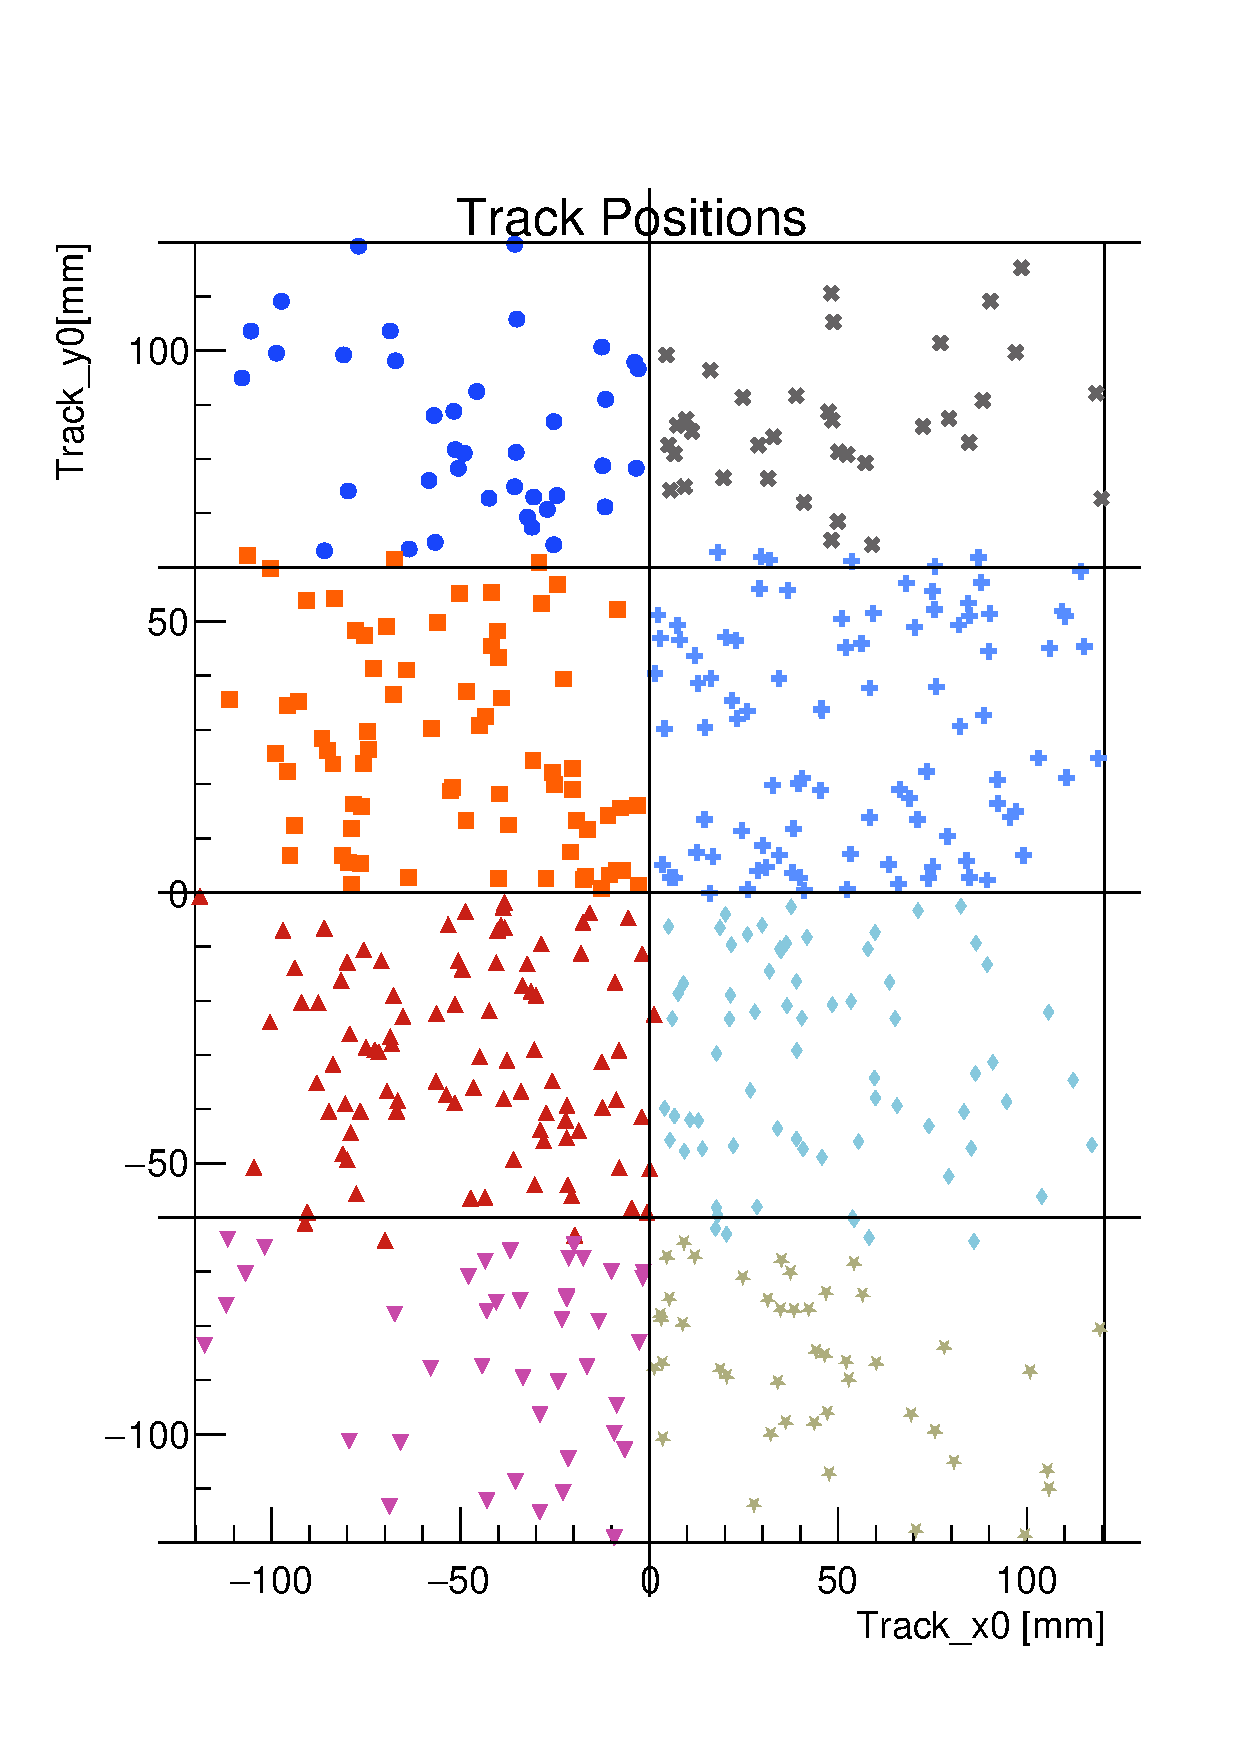
\includegraphics[height=0.8\textheight]{./ModuleLevelPlots/Positions_st0_truemodule0.pdf}
%                 \caption{500 Points at Station-1 colored according to module-variables in 2024 data}
%             \end{figure}
%         \end{column}
%         \begin{column}{0.2\linewidth}
%             \begin{figure}
%                 \hspace{-7cm}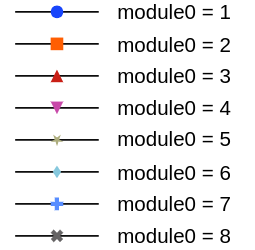
\includegraphics[scale=0.25]{./assets/image.png}
%             \end{figure}
%         \end{column}
%     \end{columns}
% \end{frame}

% \begin{frame}{Where are the Module Boundaries?}
%     \begin{columns}
%         \begin{column}{0.5 \linewidth}
%             \begin{figure}
%                 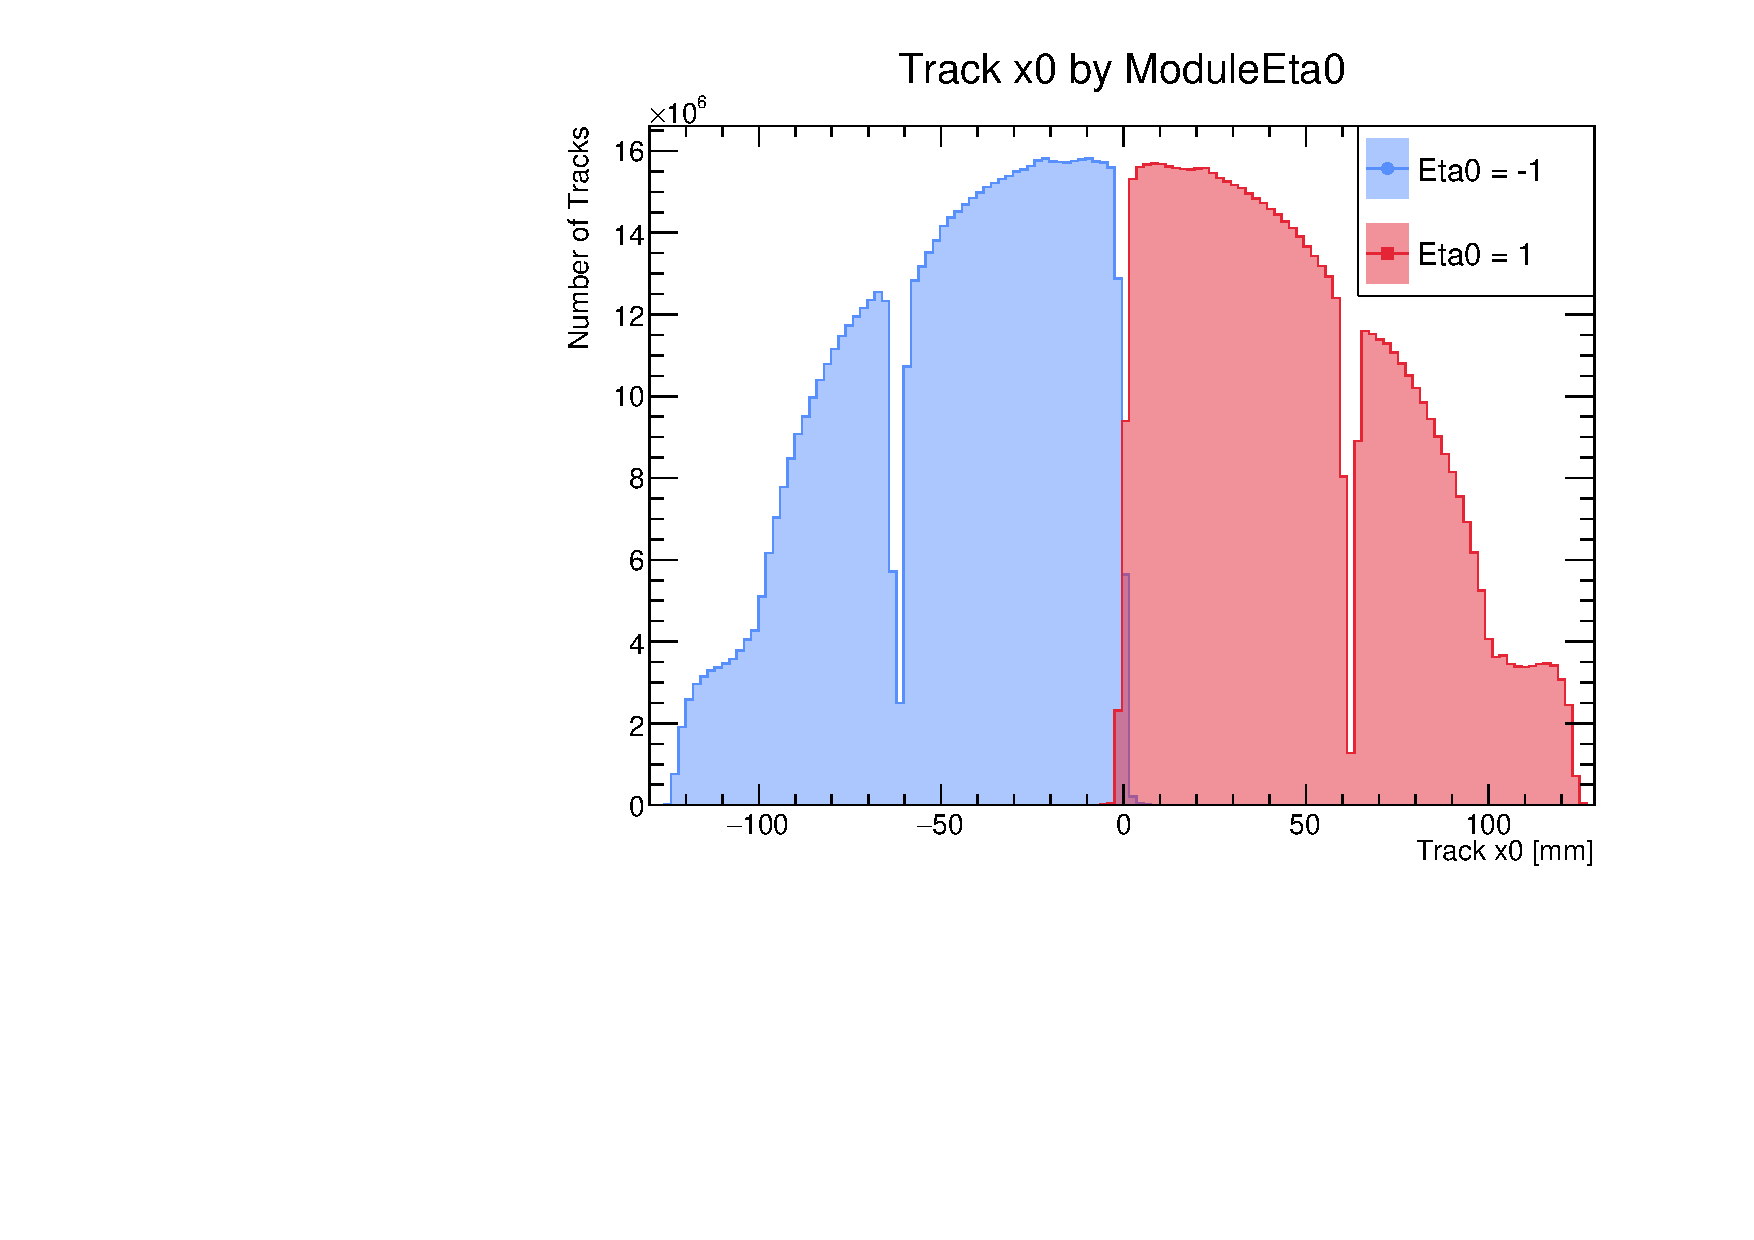
\includegraphics[width=\linewidth]{./ModuleLevelPlots/Track_x0_eta0.pdf}
%                 \caption{Track Positions at Station 1 colored by module\_eta0}
%             \end{figure}
%         \end{column}
%         \begin{column}{0.5 \linewidth}
%             \begin{figure}
%                 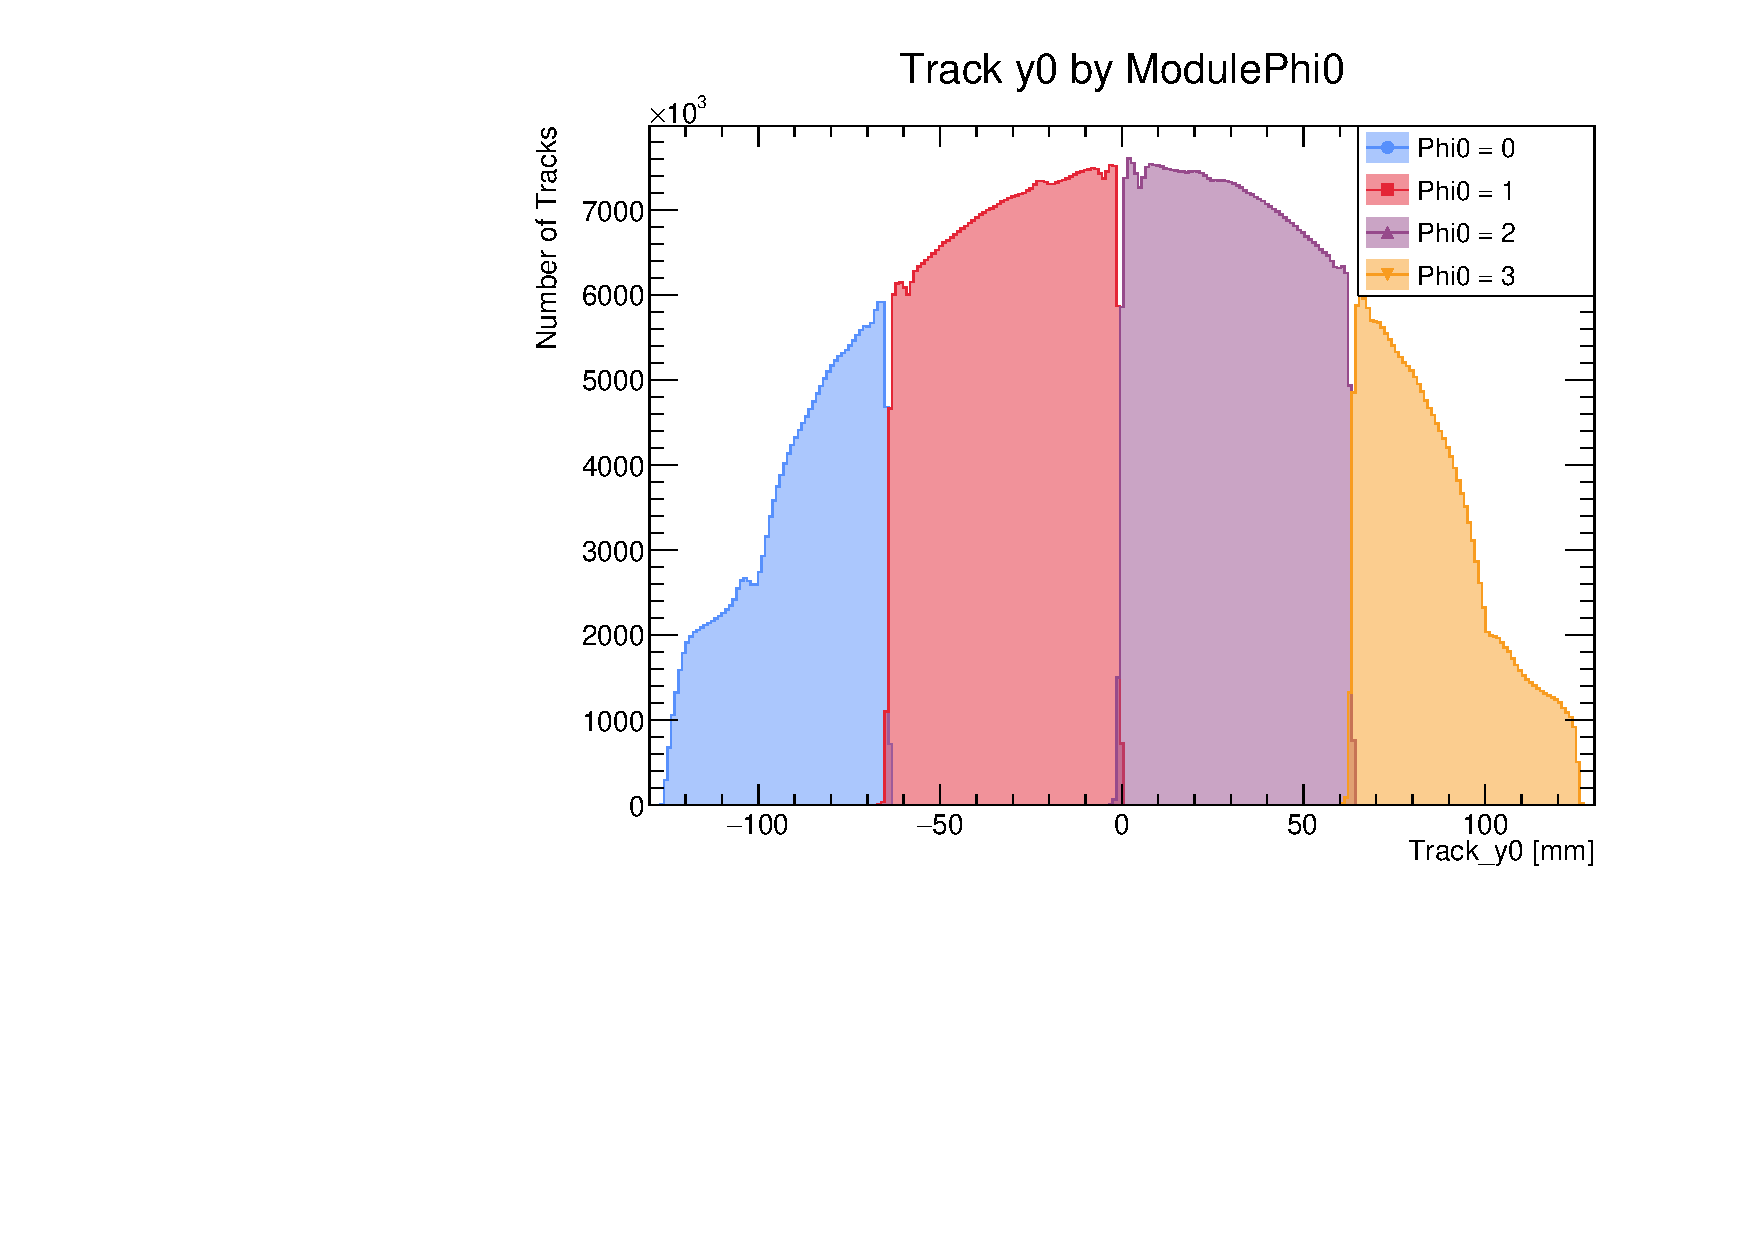
\includegraphics[width=\linewidth]{./ModuleLevelPlots/Track_y0_phi0.pdf}
%                 \caption{Track Positions at Station 1 colored by module\_phi0}
%             \end{figure}
%         \end{column}
%      \end{columns}
% \end{frame}




% \begin{frame}{Accuracy of Module Splits}
%     \begin{itemize}
%         \item Since 2023 does not have the module\_eta0 / phi0 entries we approximate them using the above schematic.
%     \end{itemize}
%     \begin{figure}
%         \centering
%         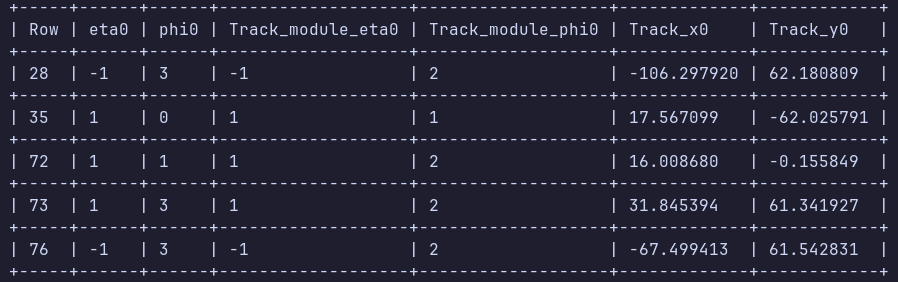
\includegraphics[width=1.0\linewidth]{./assets/ModuleMismatch.png}
%         \caption{Module Calculation mismatch in run 016635}
%     \end{figure}   
%     \begin{itemize}
%         \item Mismatch are within $\pm$ 5 mm of the borders
%         \item Number of Mismatches:  587982  out of  13601766 i.e 4.3\%
%     \end{itemize}
% \end{frame}

\begin{frame}{Revisiting Positions at Station 1}
    \begin{columns}
        \begin{column}{1.2\linewidth}
            \begin{figure}
                \centering
                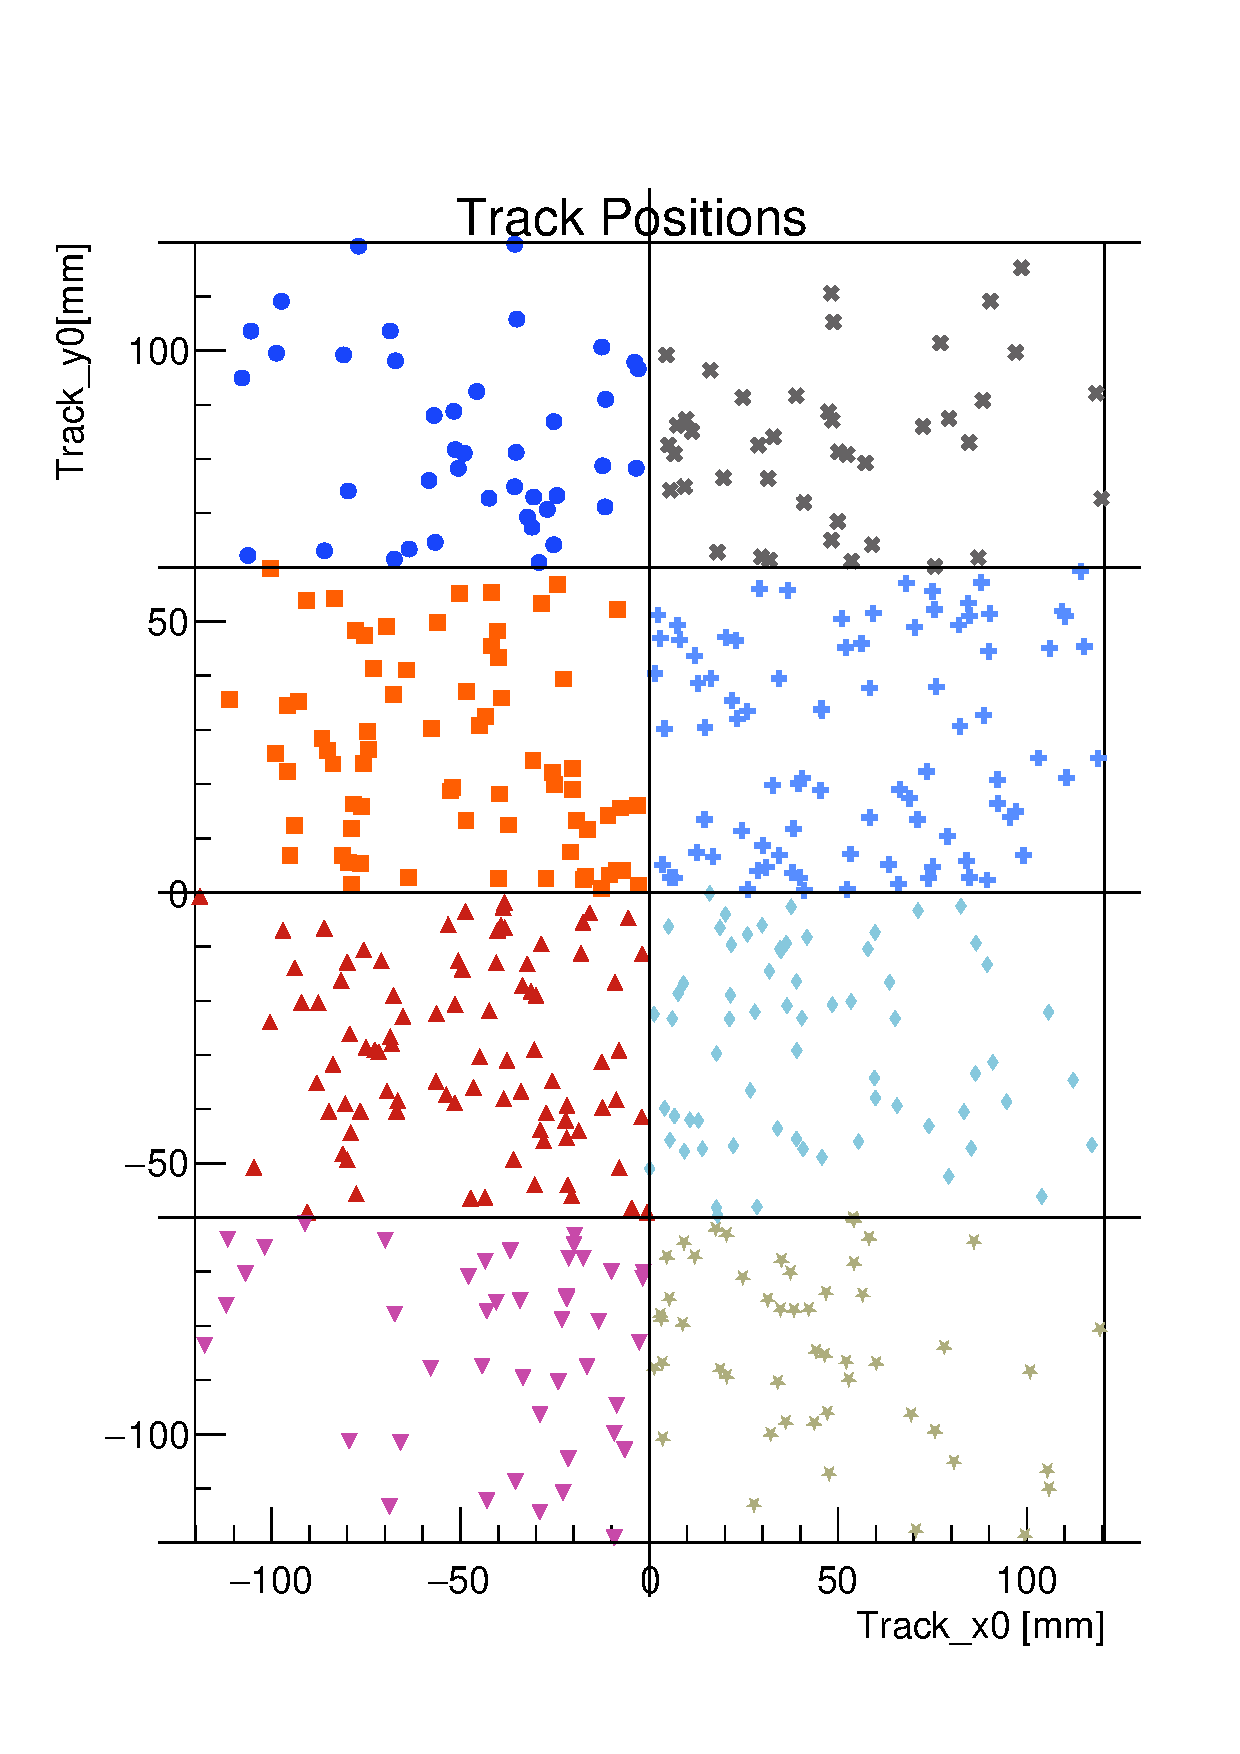
\includegraphics[height=0.8\textheight]{./ModuleLevelPlots/Positions_st0_module0.pdf}
                \caption{500 Points at Station 1 colored by Module number (estimated) at Station 1 for 2024 data}
            \end{figure}
        \end{column}
        \begin{column}{0.2\linewidth}
            \begin{figure}
                \hspace{-7cm}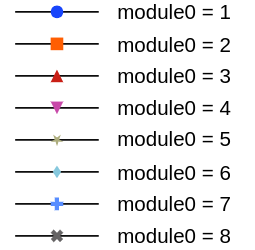
\includegraphics[scale=0.25]{./assets/image.png}
            \end{figure}
        \end{column}
    \end{columns}
\end{frame}

\begin{frame}{Where do they end up in Station 3?}
    \begin{columns}
        \begin{column}{1.2\linewidth}
            \begin{figure}
                \centering
                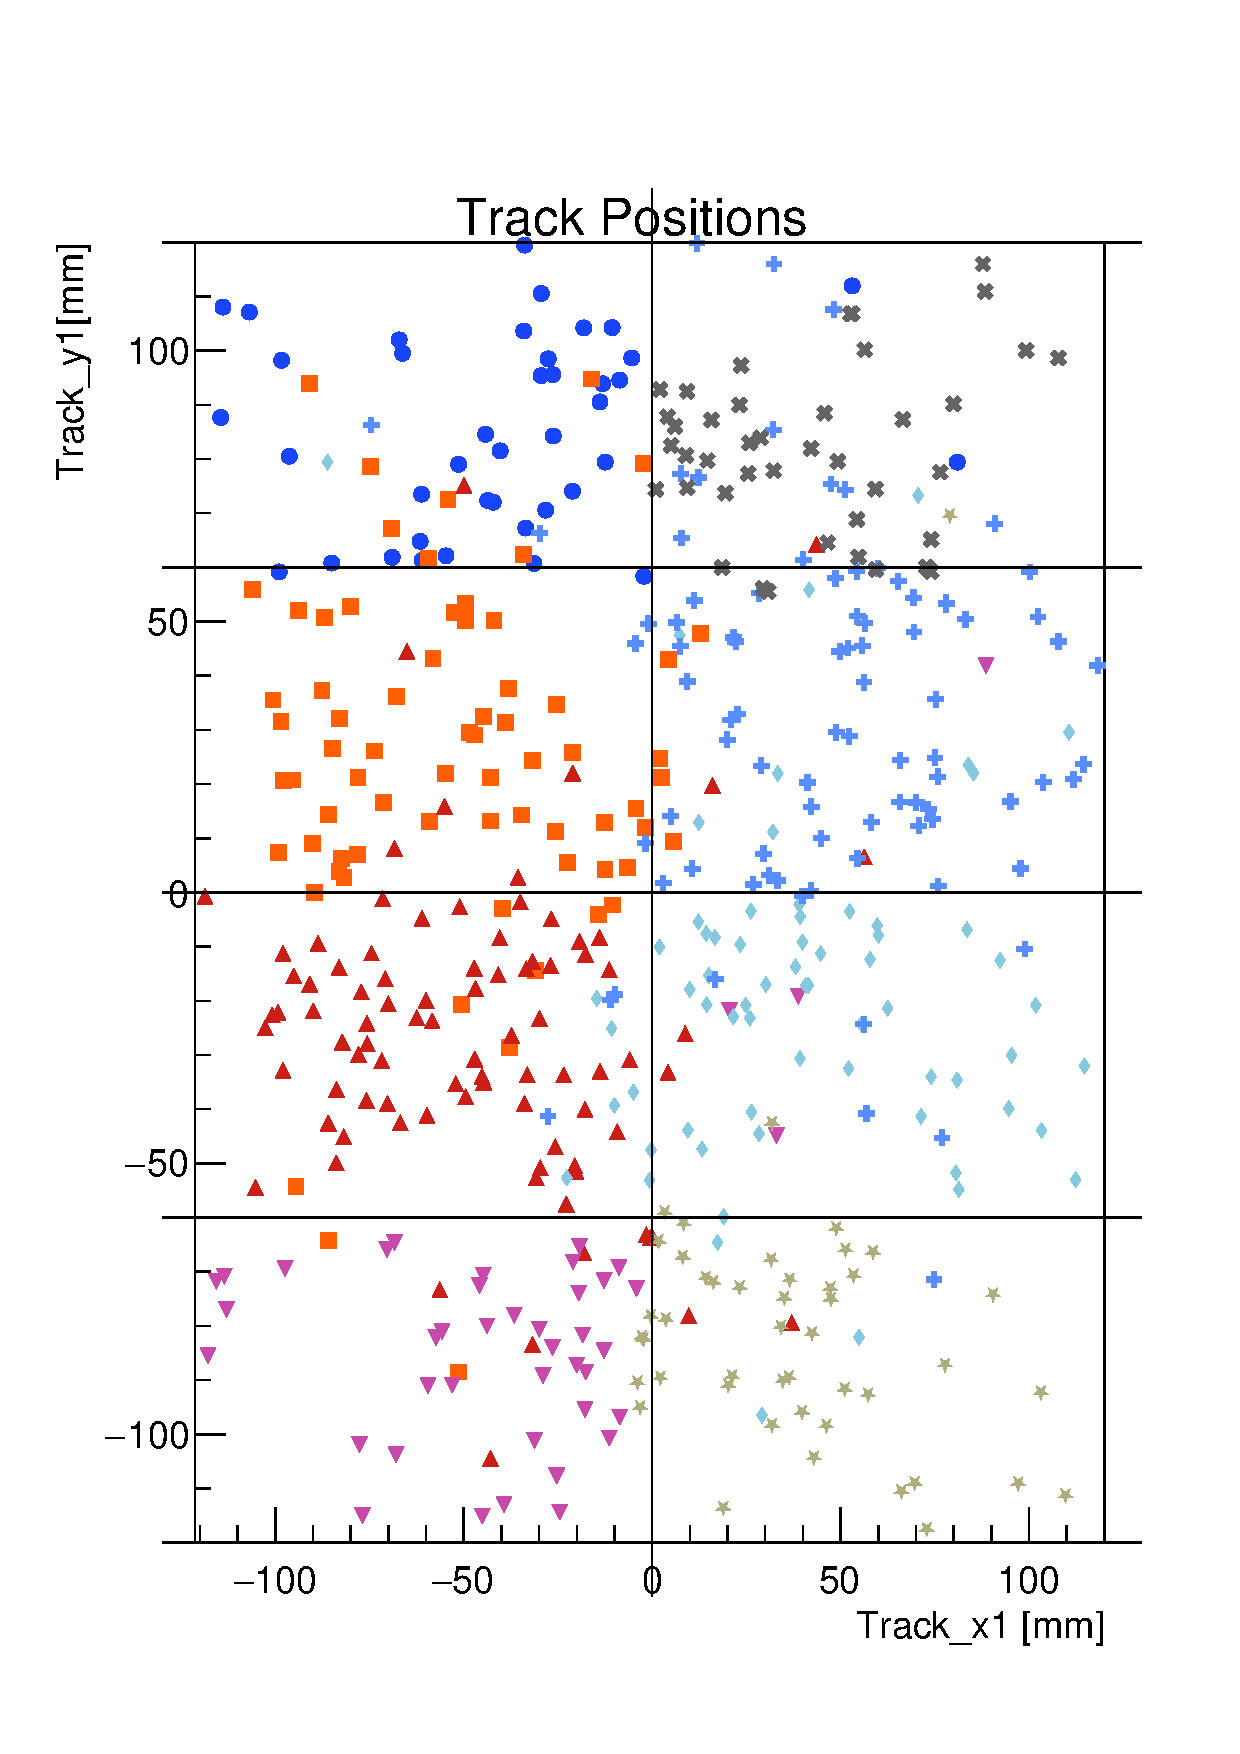
\includegraphics[height=0.8\textheight]{./ModuleLevelPlots/Positions_st1_module0.pdf}
                \caption{500 Points at Station 3 colored by Module number at Station 1 for 2024 data [Same tracks as previous slide]}
            \end{figure}
        \end{column}
        \begin{column}{0.2\linewidth}
            \begin{figure}
                \hspace{-7cm}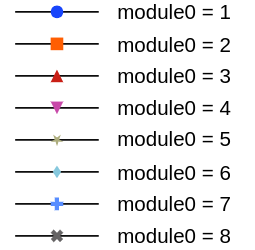
\includegraphics[scale=0.25]{./assets/image.png}
            \end{figure}
        \end{column}
    \end{columns}
\end{frame}

\begin{frame}{Transfer Heatmap in 2023}
    \begin{columns}
        \begin{column}{0.85\linewidth}
            \begin{figure}
                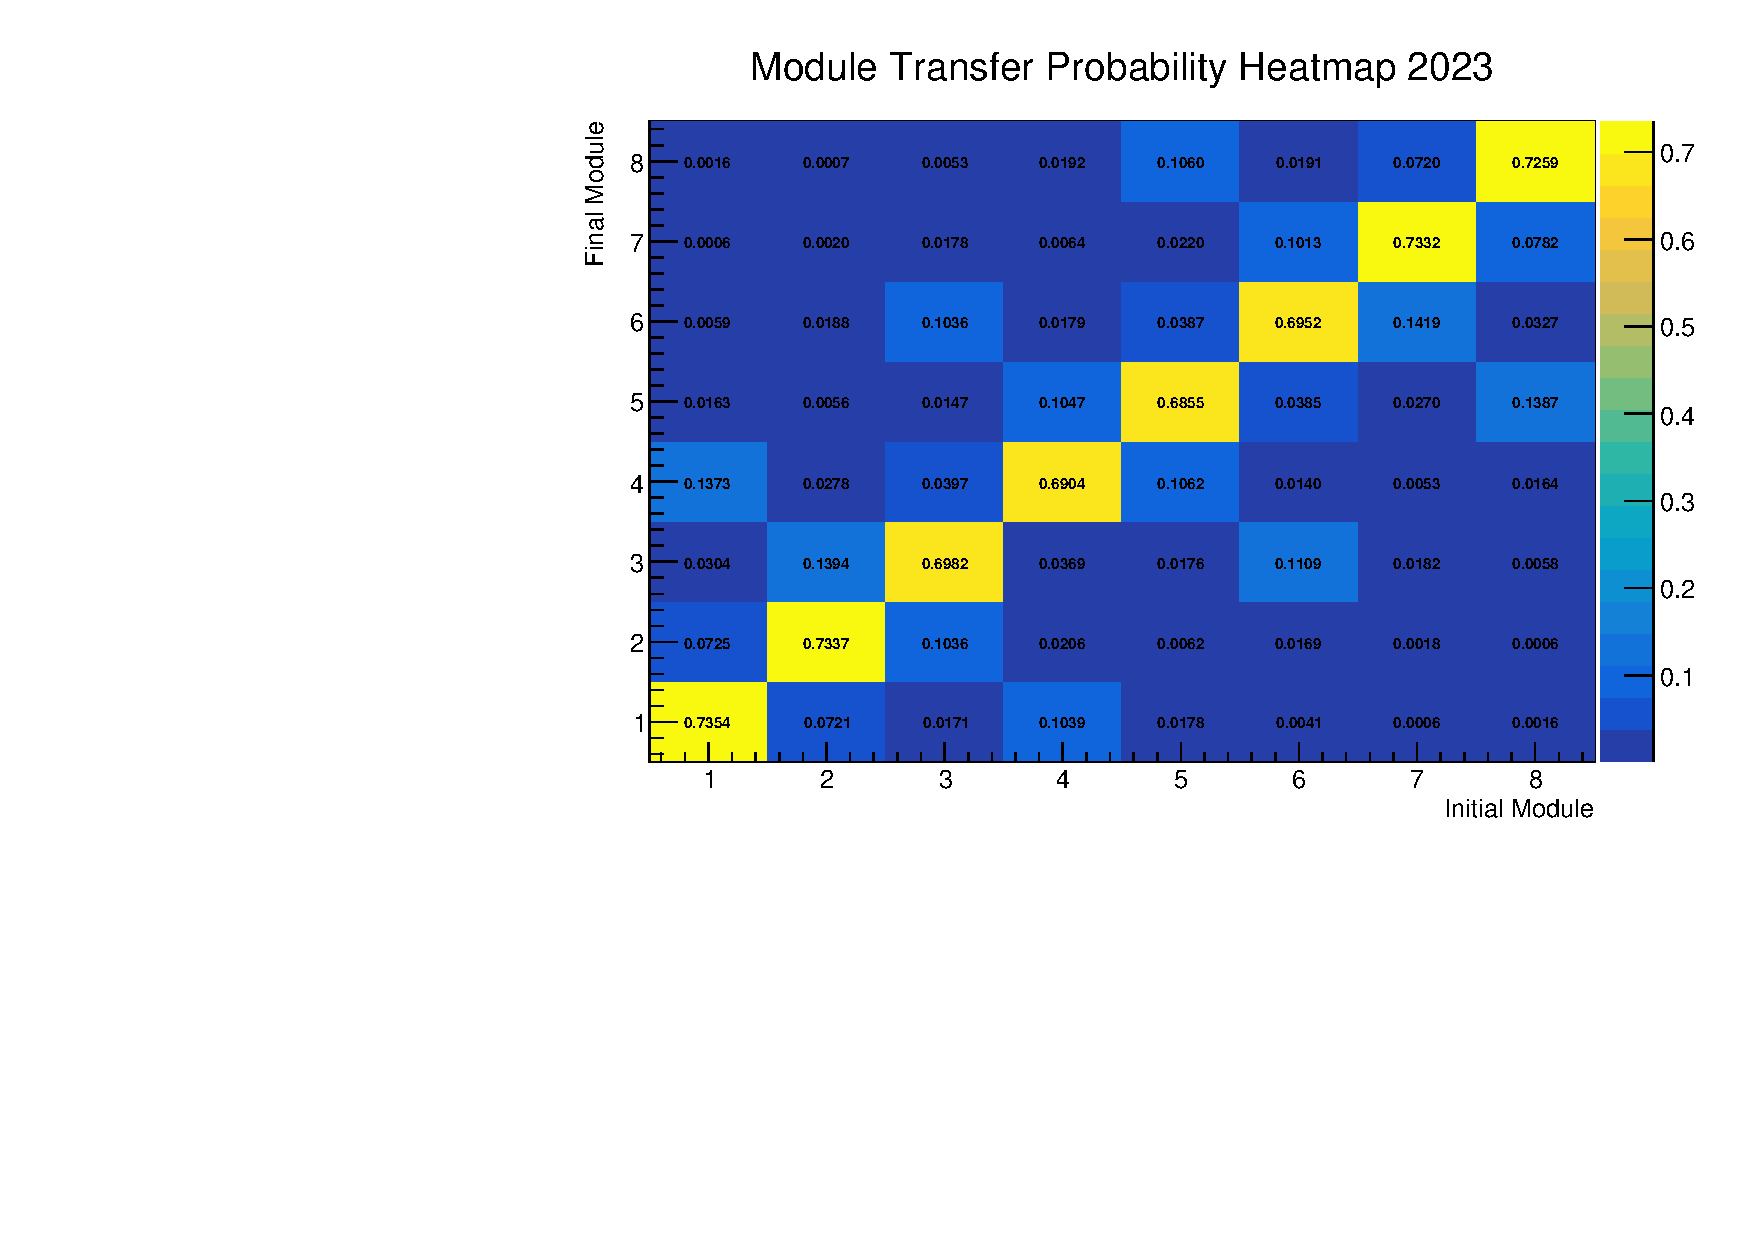
\includegraphics[width=0.9\linewidth]{./ModuleLevelPlots/st0_module_number vs st1_module_number_prob_2023.pdf}
                \caption{Probability of Transfer from Initial Module (at Station 1) to Final Module (at Station 2) based on 2023 Data}
            \end{figure}
        \end{column}
        \begin{column}{0.2\linewidth}
            \begin{figure}
                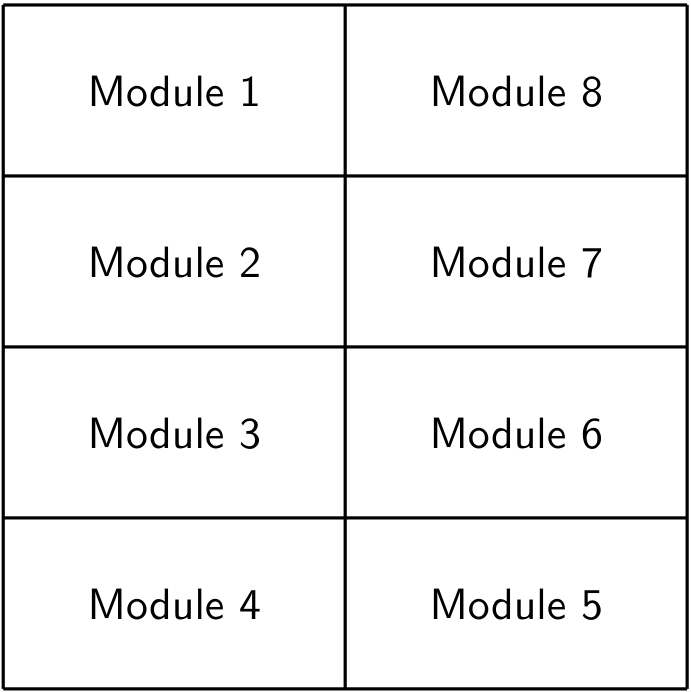
\includegraphics[width=\linewidth]{./assets/ModuleThumbnail.png}
            \end{figure}
        \end{column}
    \end{columns}
    \begin{itemize}
        \small
        \item Most probable transfer is to the same module followed by adjacent.
        \item Module 2,3,6,7 (central) are more likely to transfer to another central module. 
    \end{itemize}
\end{frame}

\begin{frame}{Transfer Heatmap in 2024}
    \begin{figure}
        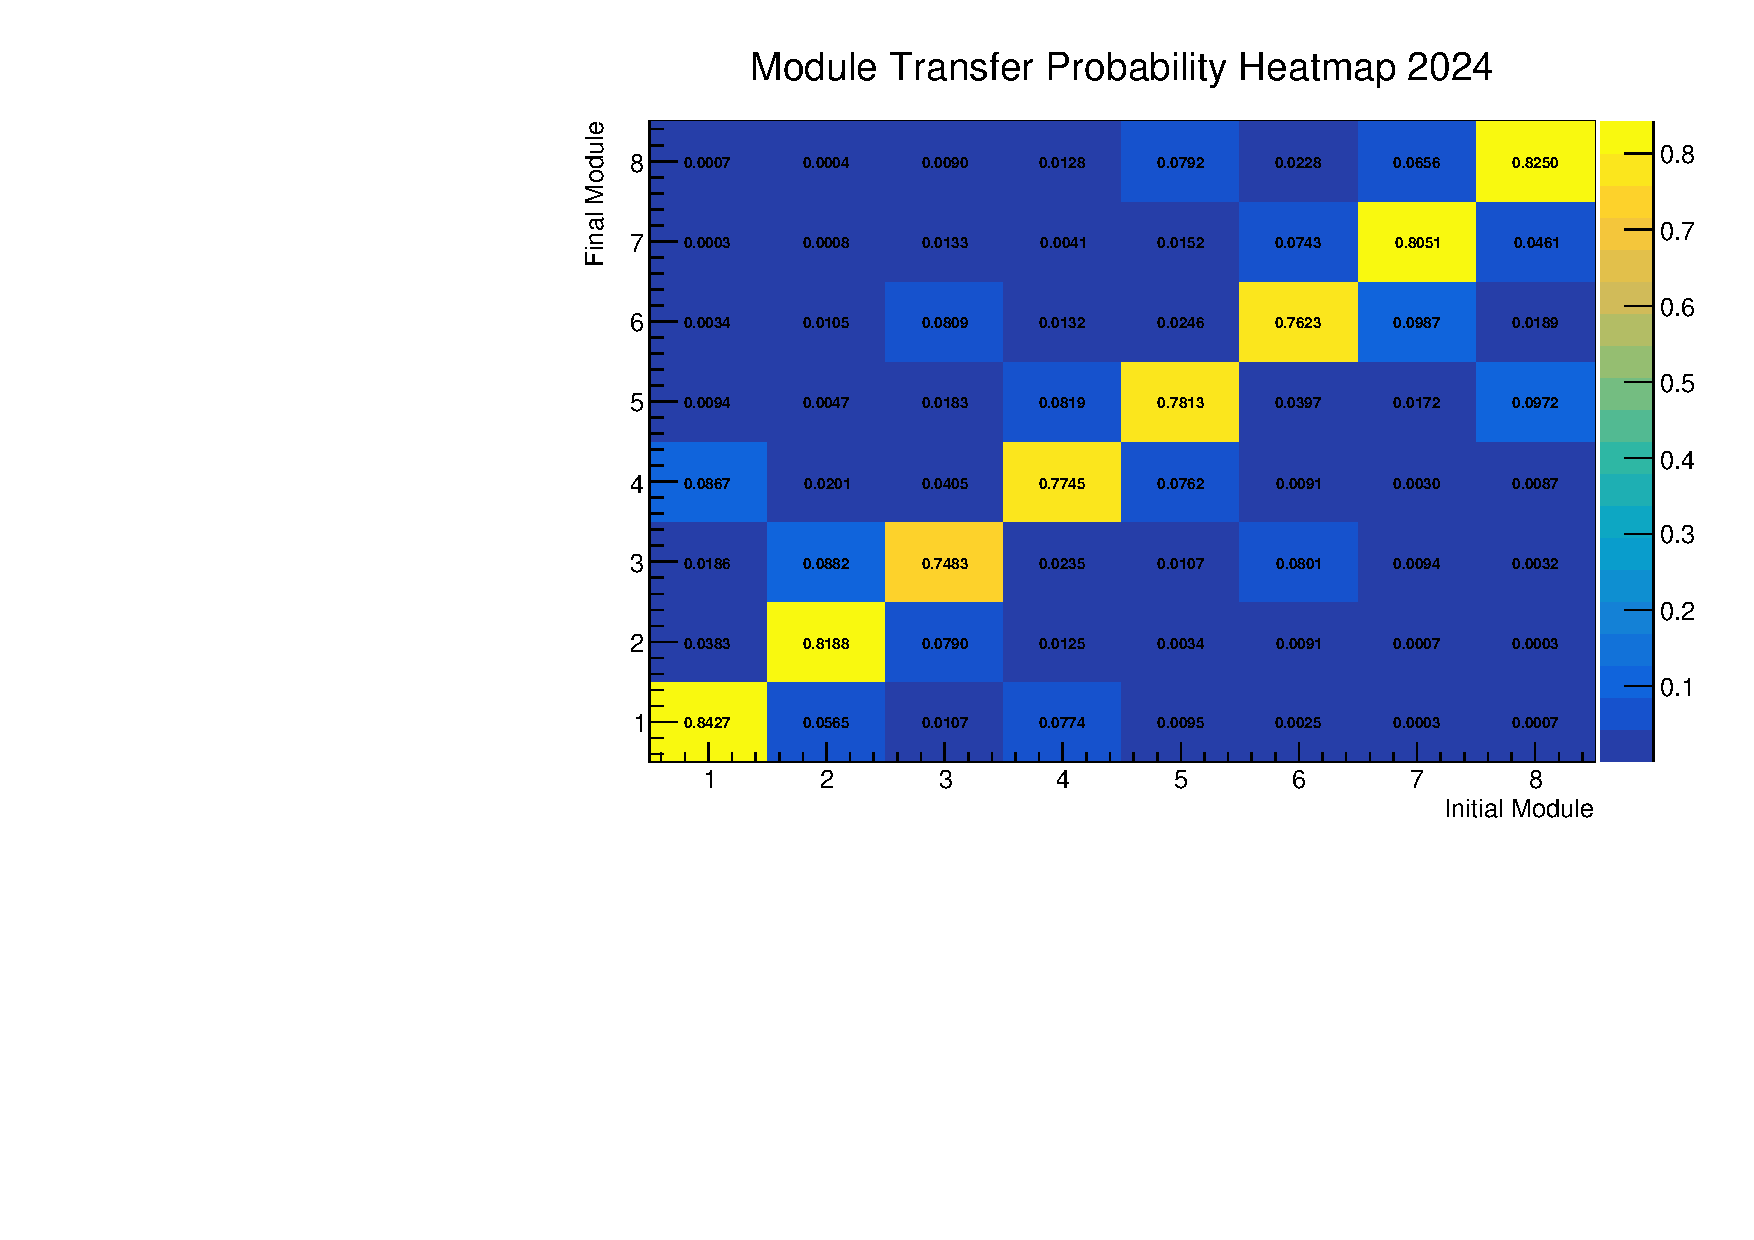
\includegraphics[width=0.8\linewidth]{./ModuleLevelPlots/st0_module_number vs st1_module_number_prob_2024.pdf}
        \caption{Probability of Transfer from Initial Module (at Station 1) to Final Module (at Station 2) based on 2024 data}
    \end{figure}
    \begin{itemize}
        \small
        \item Much higher Probability of Transfer to the same module
        \item In general less module transfers in 2024. [Higher Momentum Tracks]
    \end{itemize}
\end{frame}

\begin{frame}{Transfer Heatmap Ratio }
    \begin{figure}
        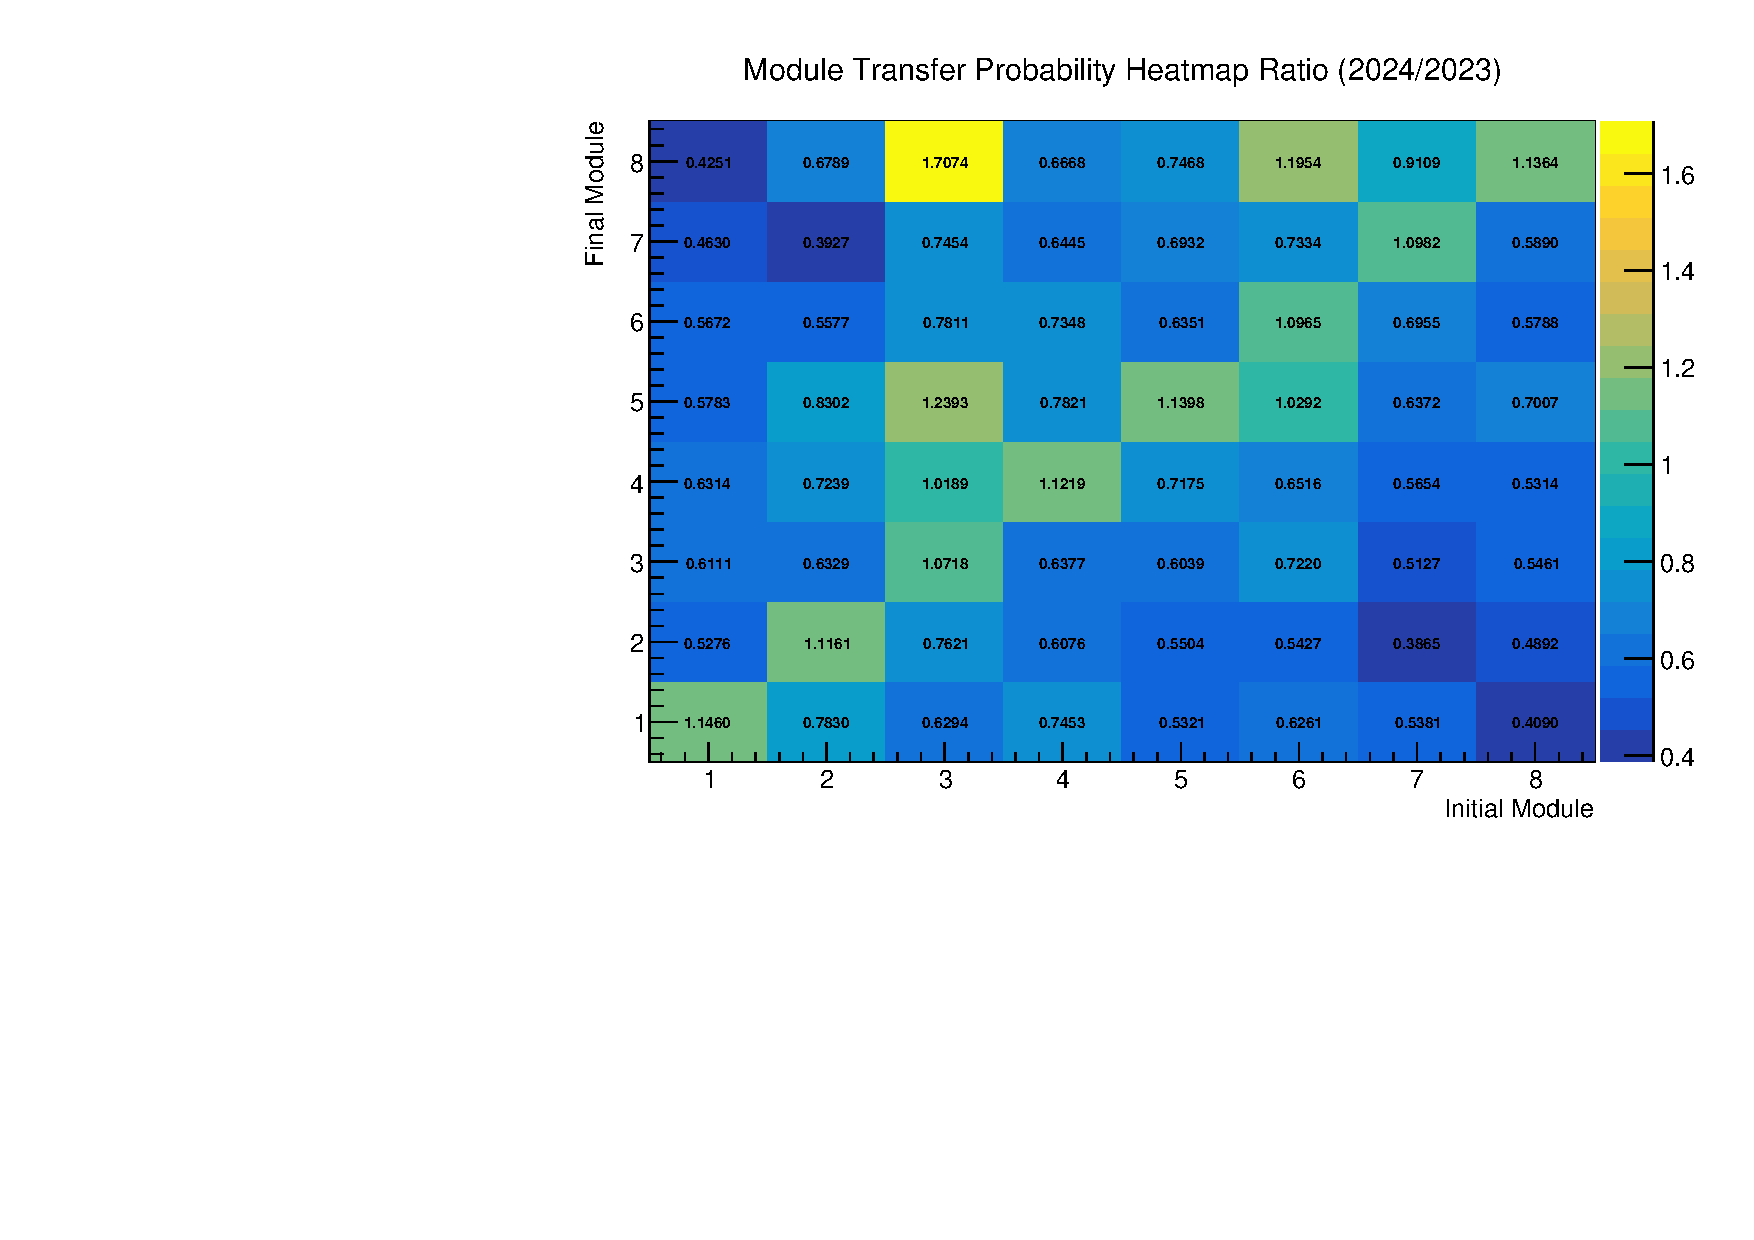
\includegraphics[width=0.86\linewidth]{./ModuleLevelPlots/st0_module_number vs st1_module_number_prob_ratio.pdf}
        \caption{Ratio of Probability of Transfer from Initial Module (at Station 1) to Final Module (at Station 2) }
    \end{figure}
    \begin{itemize}
        \small
        \item 2024 has a higher probability of transfer to the same module
        \item Module 3 and 6 seem to be transferring into 8 more [Why?]
    \end{itemize}

\end{frame}


% \begin{frame}{Transfer Histograms}
%     \begin{figure}
%         \centering
%         \begin{subfigure}[t]{0.49\linewidth}
%             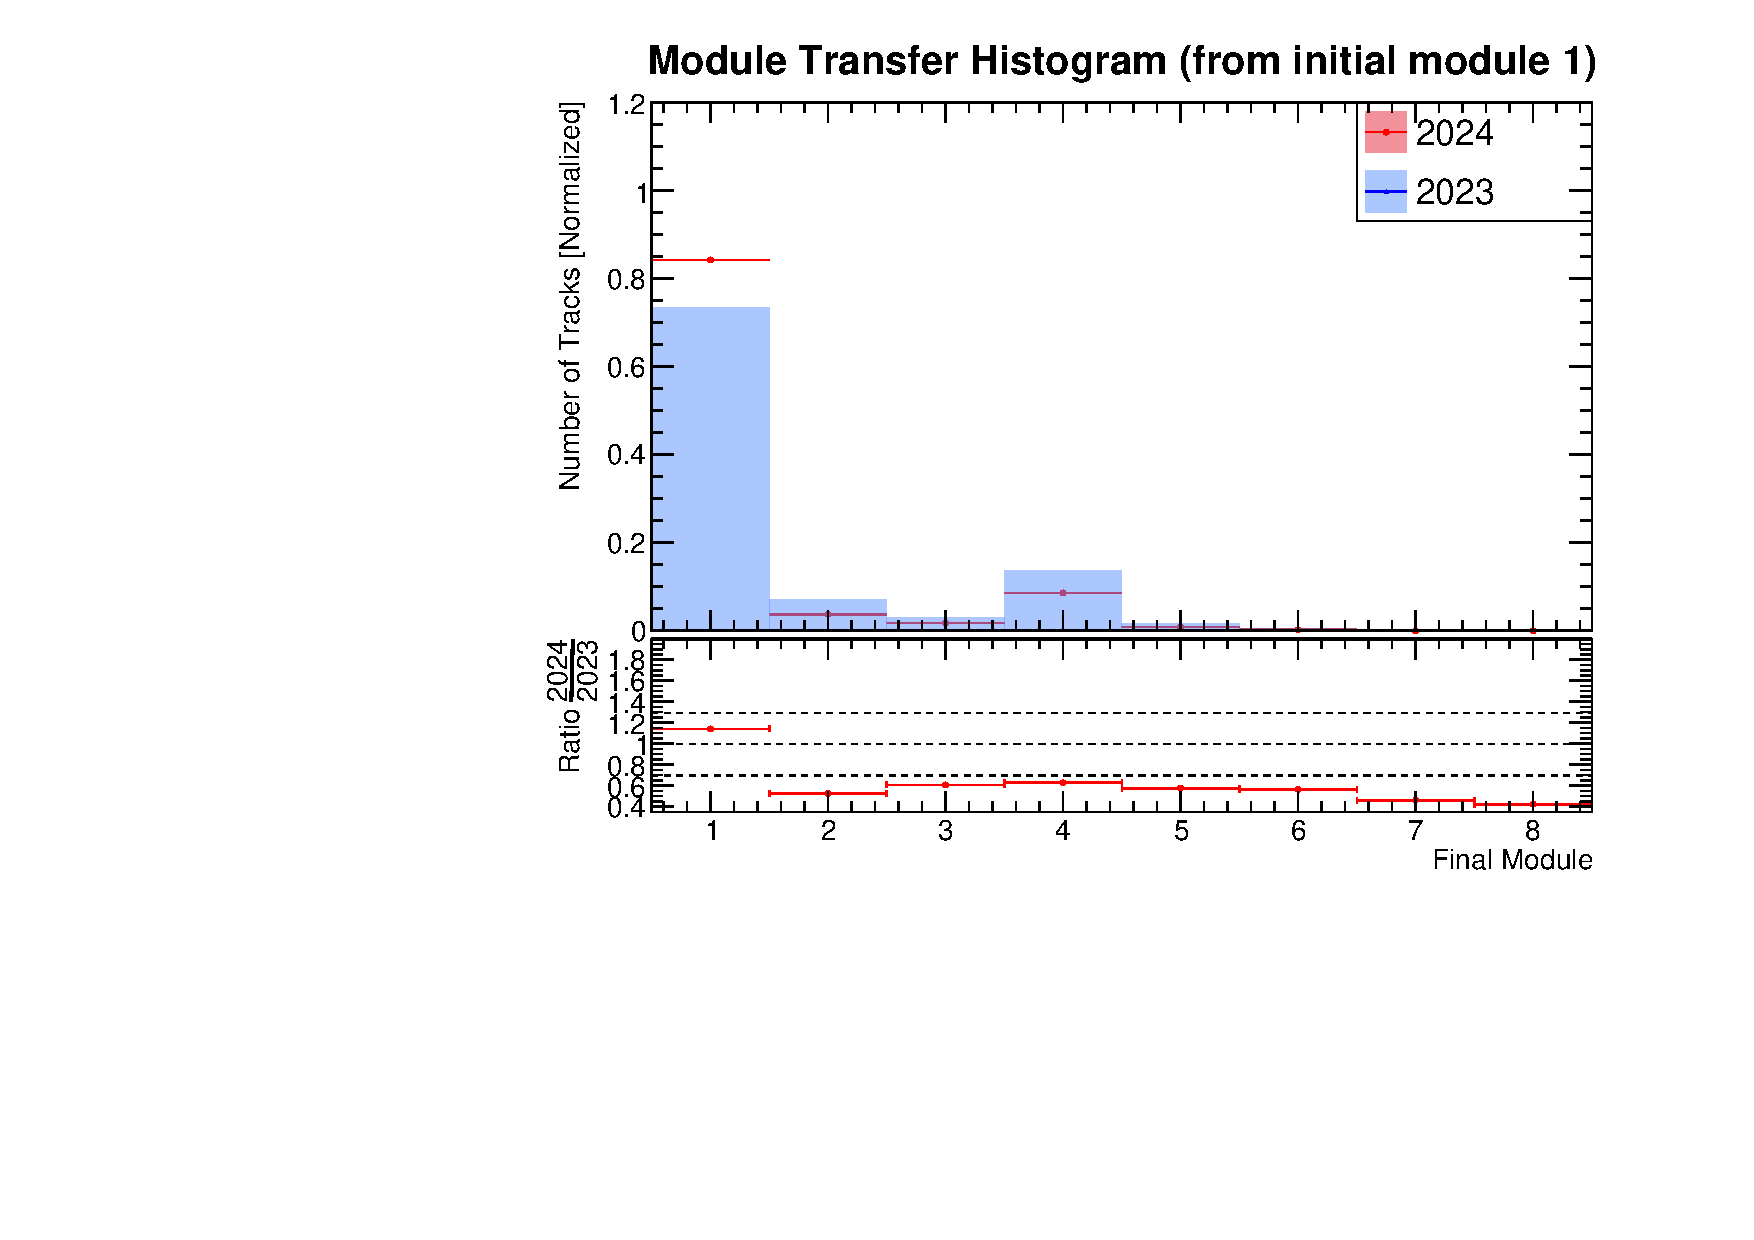
\includegraphics[width=\linewidth]{./ModuleLevelPlots/final_module_from_st0_module1.pdf}
%         \end{subfigure}
%         \begin{subfigure}[t]{0.49\linewidth}
%             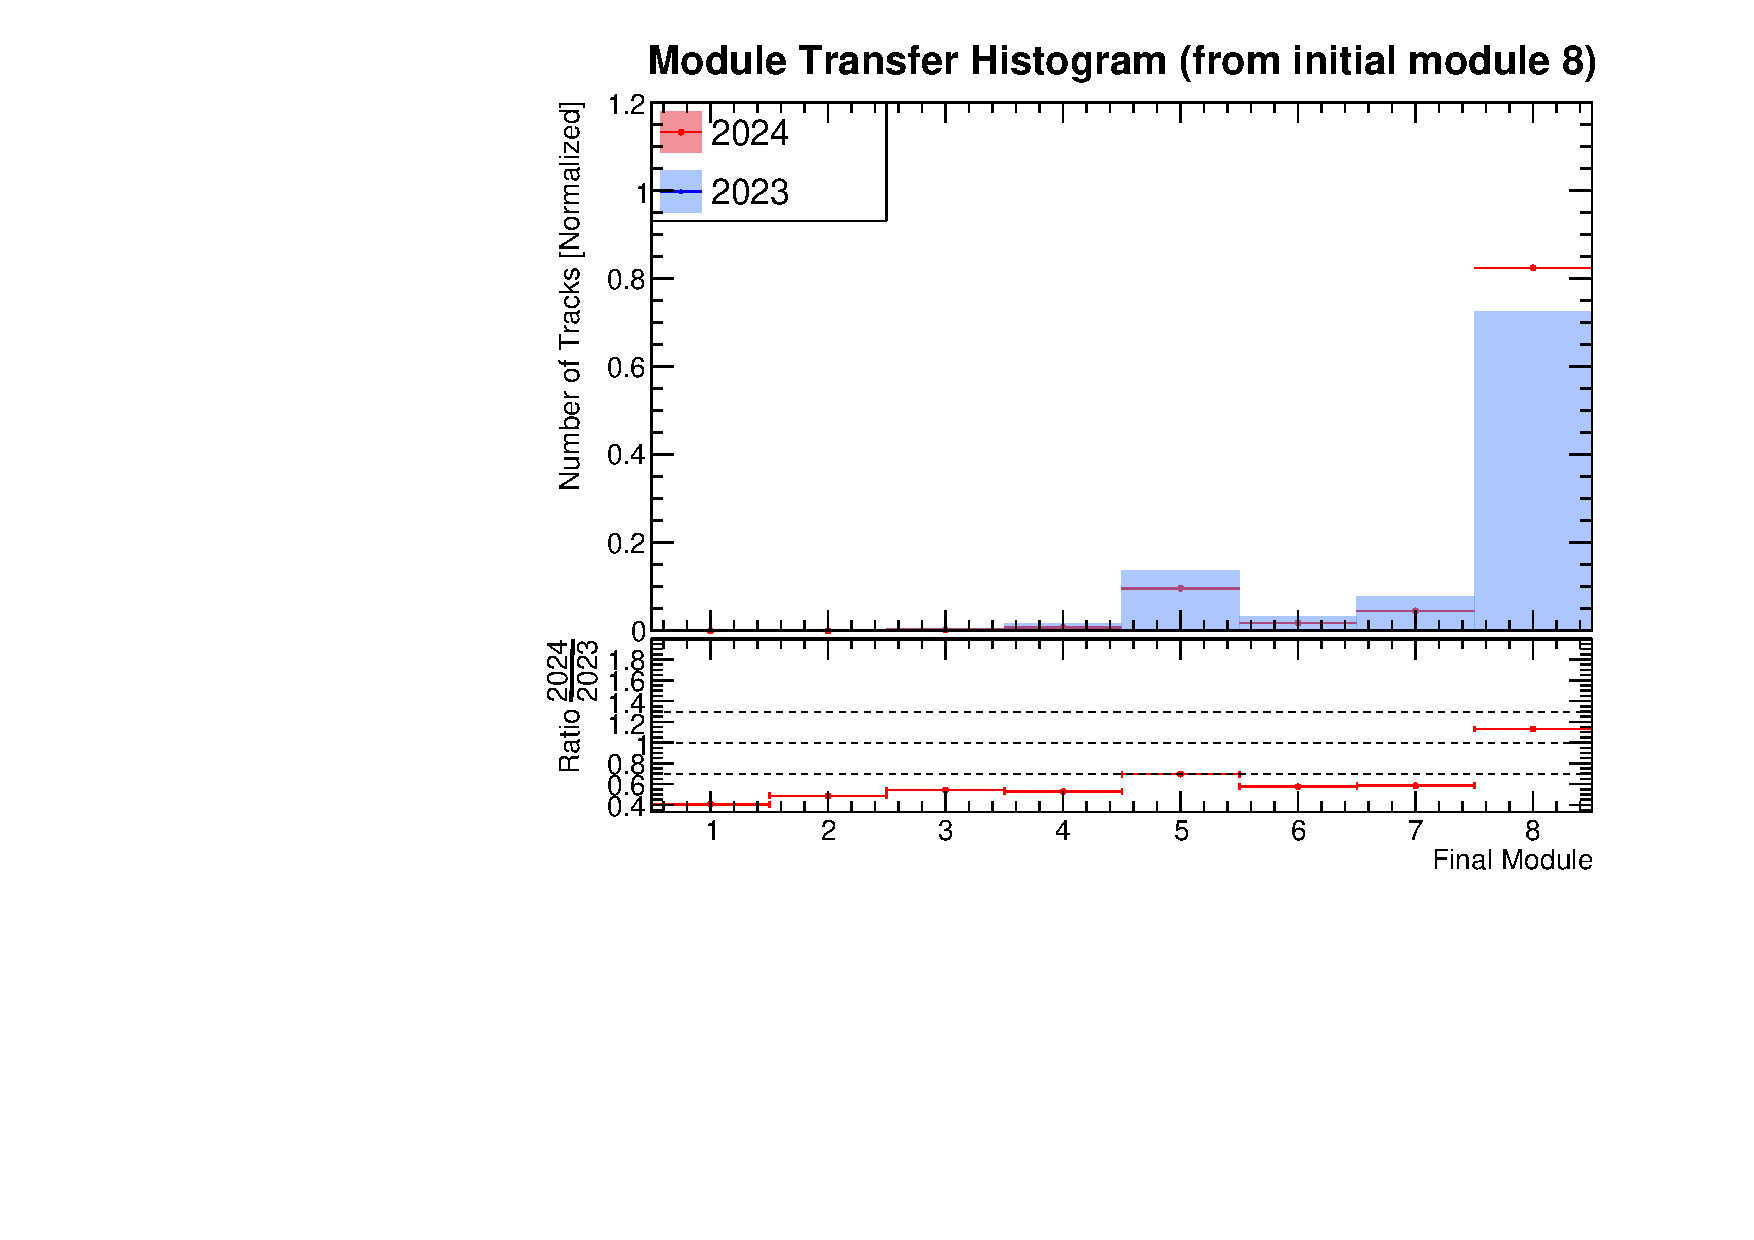
\includegraphics[width=\linewidth]{./ModuleLevelPlots/final_module_from_st0_module8.pdf}
%         \end{subfigure}

%         \begin{subfigure}[t]{0.49\linewidth}
%             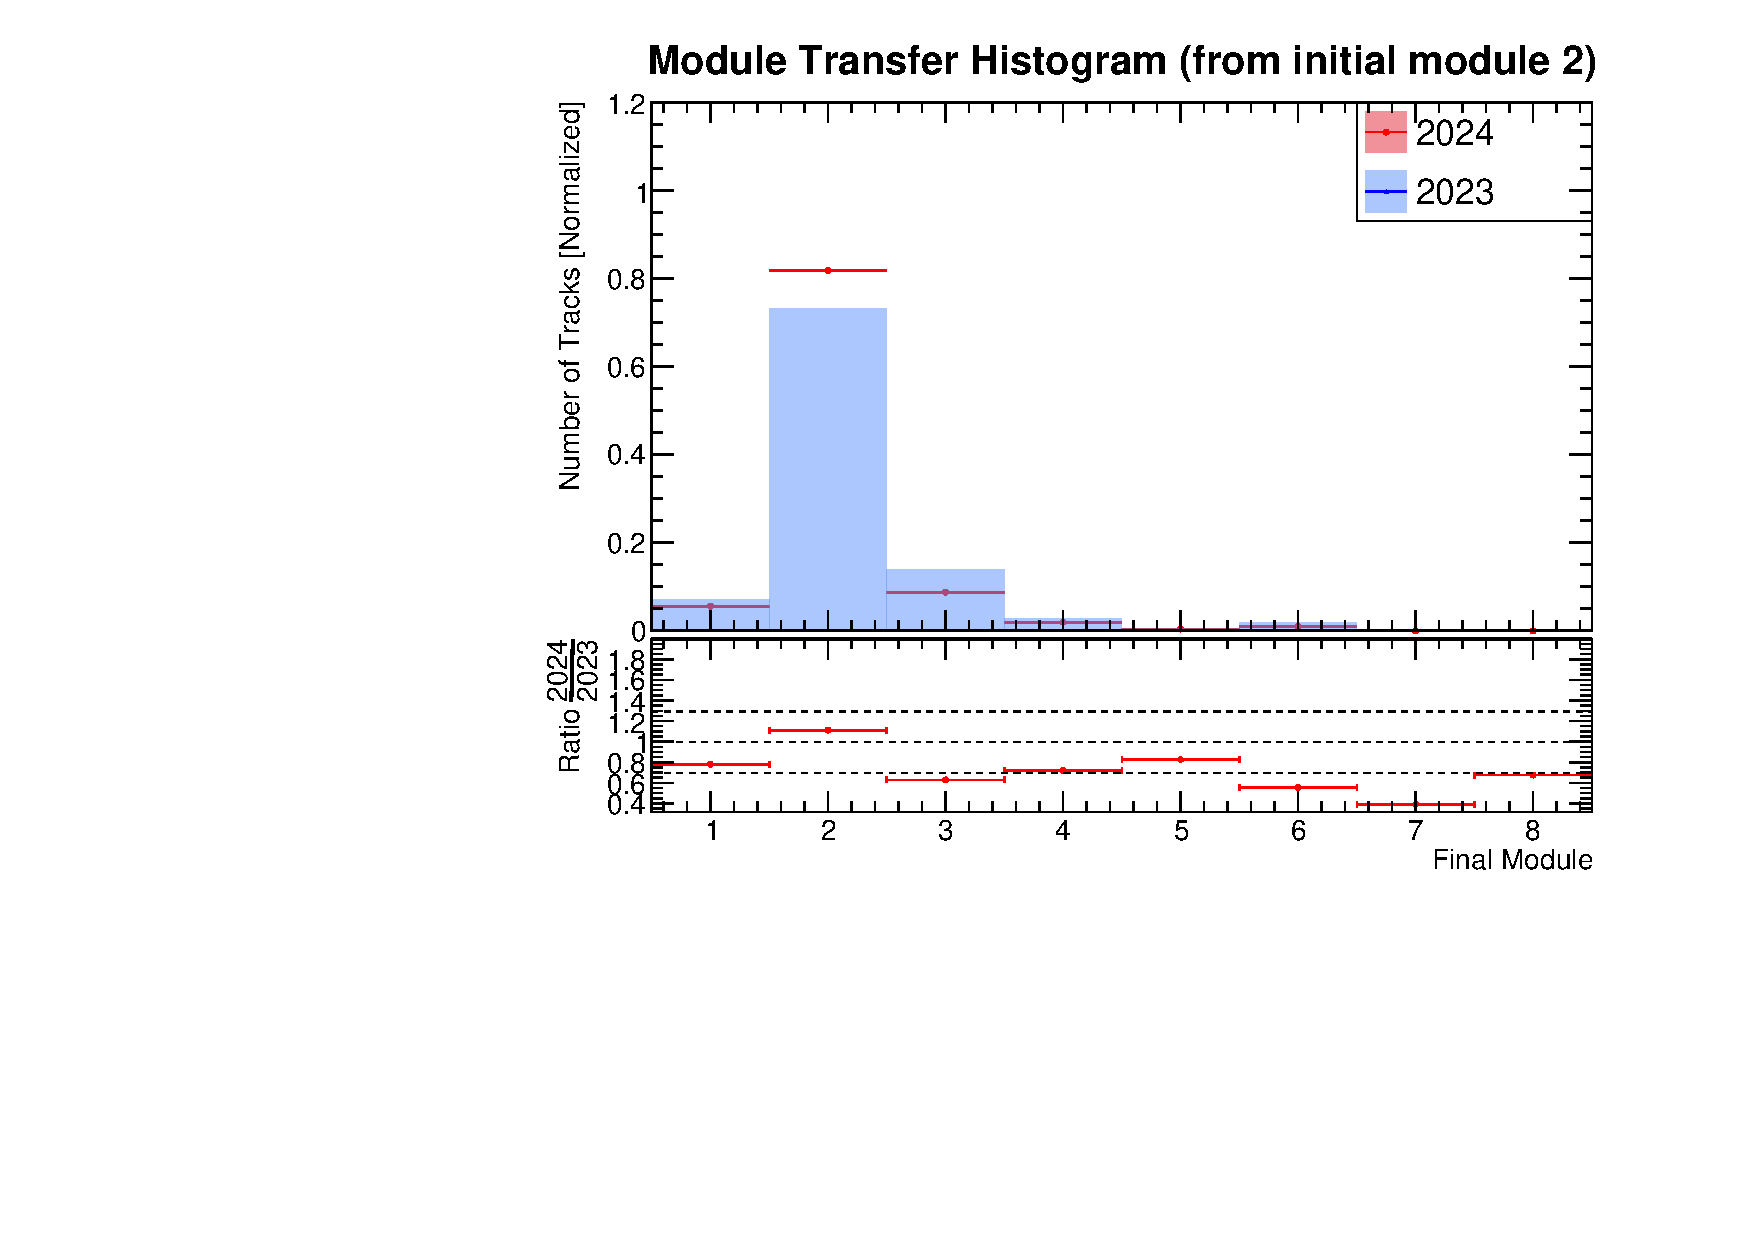
\includegraphics[width=\linewidth]{./ModuleLevelPlots/final_module_from_st0_module2.pdf}
%         \end{subfigure}
%         \begin{subfigure}[t]{0.49\linewidth}
%             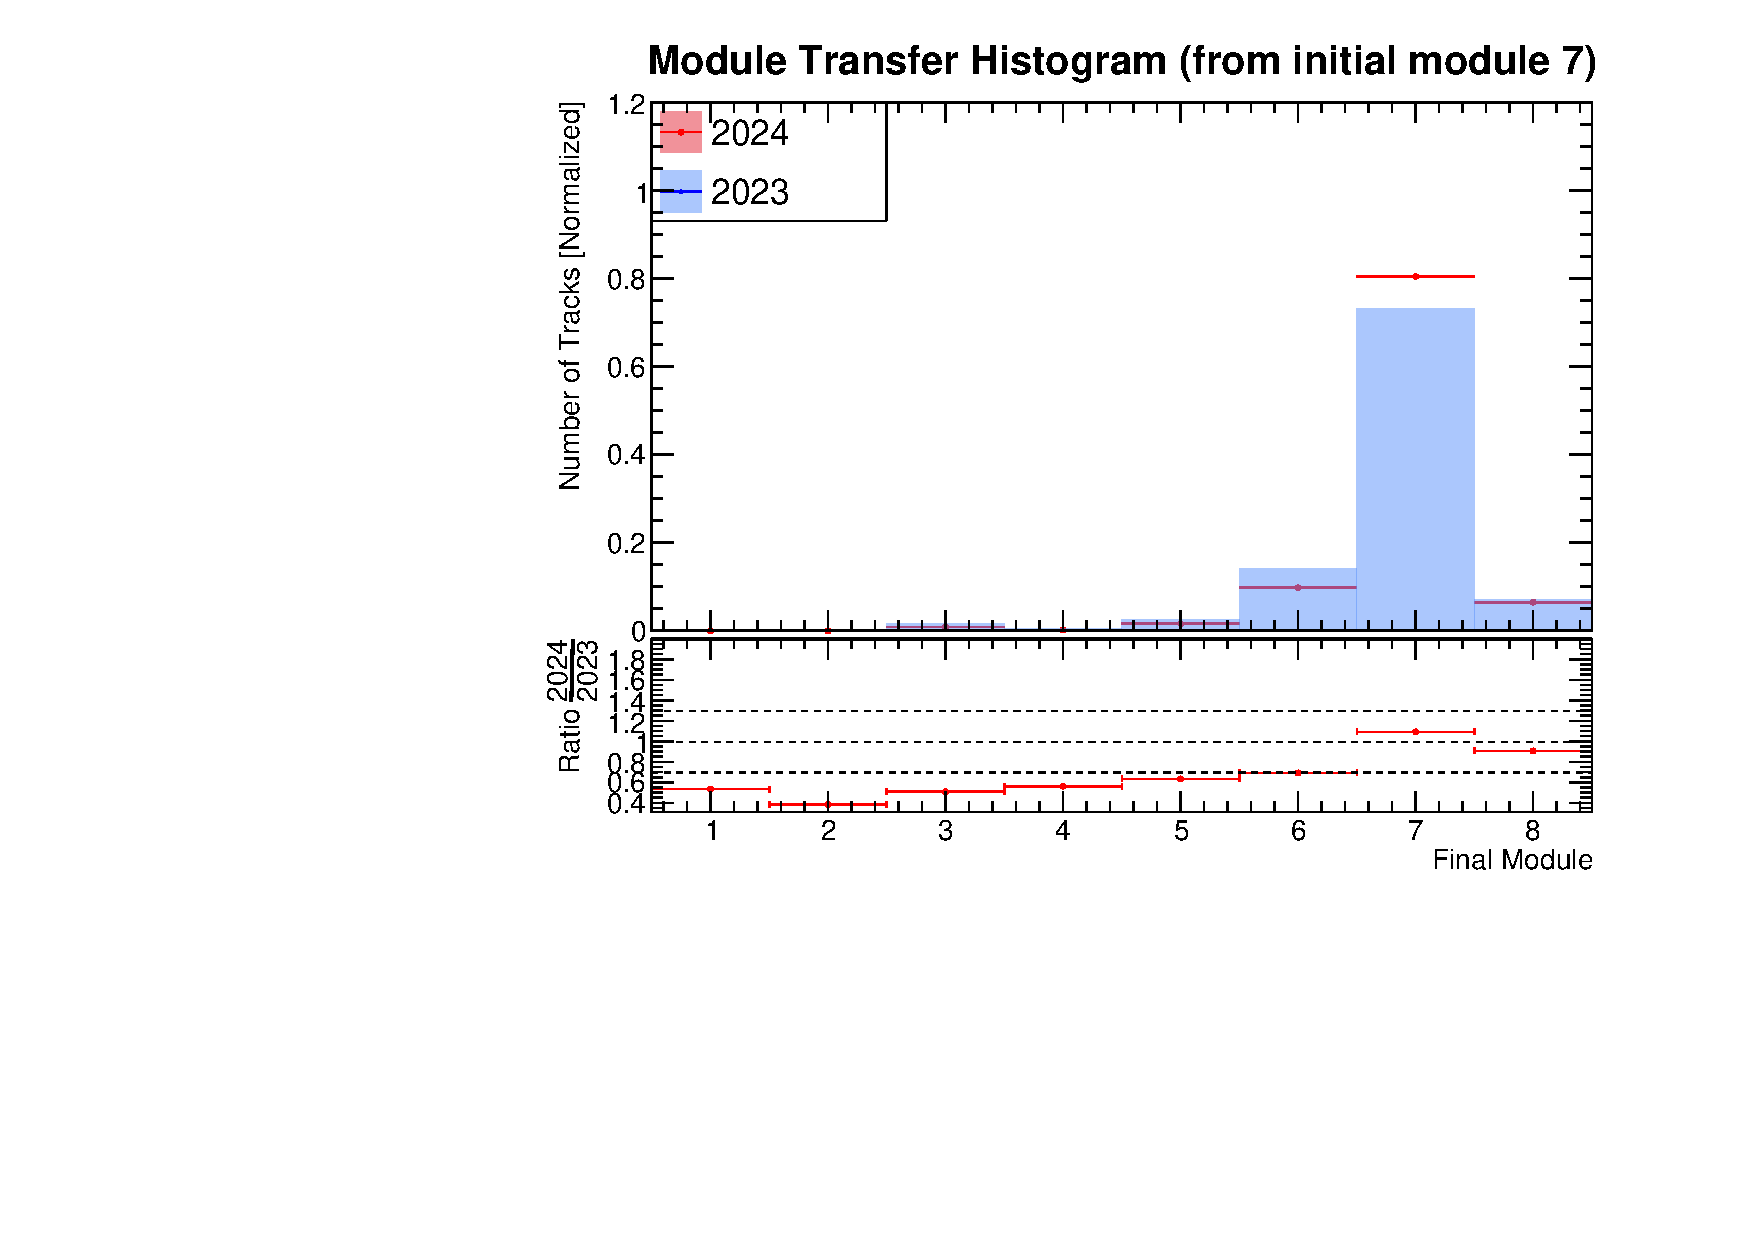
\includegraphics[width=\linewidth]{./ModuleLevelPlots/final_module_from_st0_module7.pdf}
%         \end{subfigure}
%     \end{figure}
%     \vspace{-0.3cm}
%     \scriptsize Note: 1-4 transfer seem significant? and 8-5 transfer seem significant?
% \end{frame}

% \begin{frame}{Transfer Histograms [Contd.]}
%     \begin{figure}
%         \centering
%         \begin{subfigure}[t]{0.49\linewidth}
%             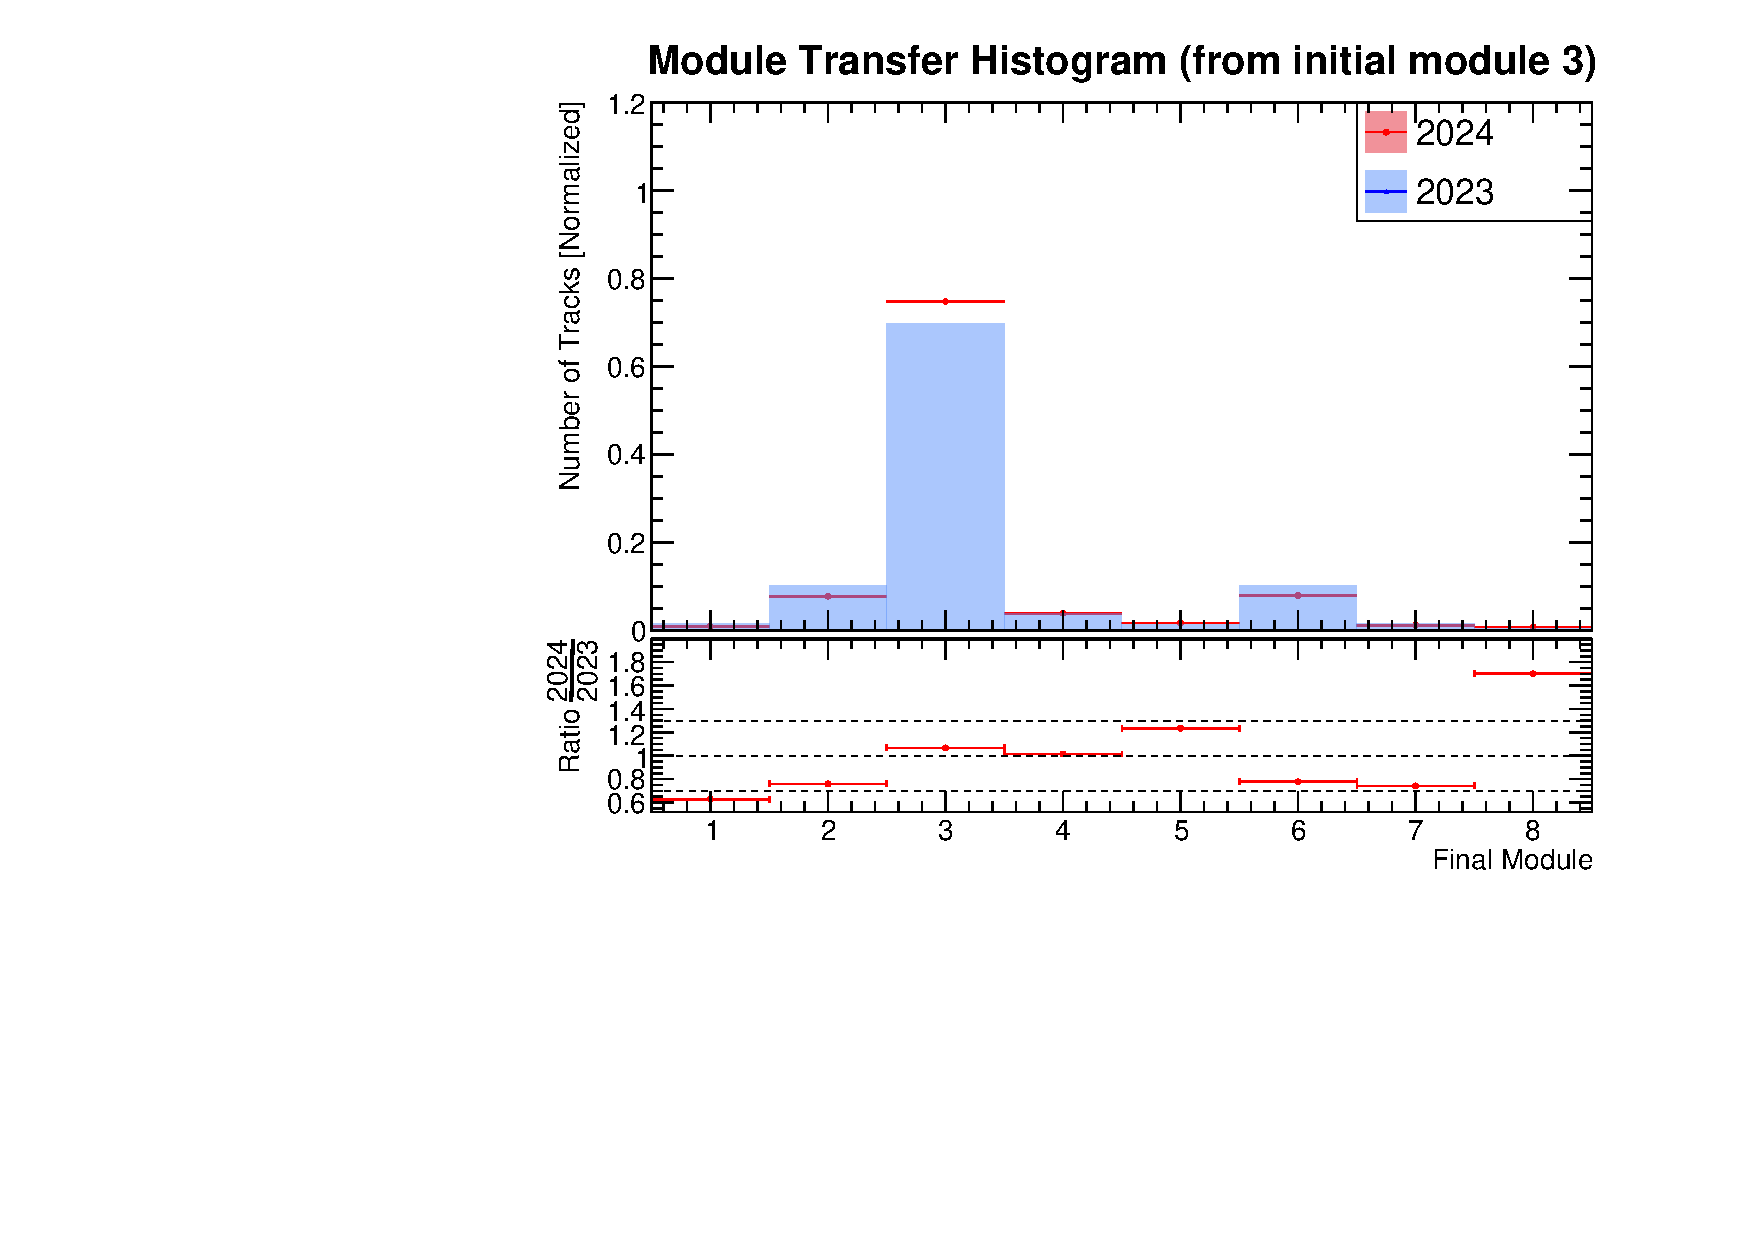
\includegraphics[width=\linewidth]{./ModuleLevelPlots/final_module_from_st0_module3.pdf}
%         \end{subfigure}
%         \begin{subfigure}[t]{0.49\linewidth}
%             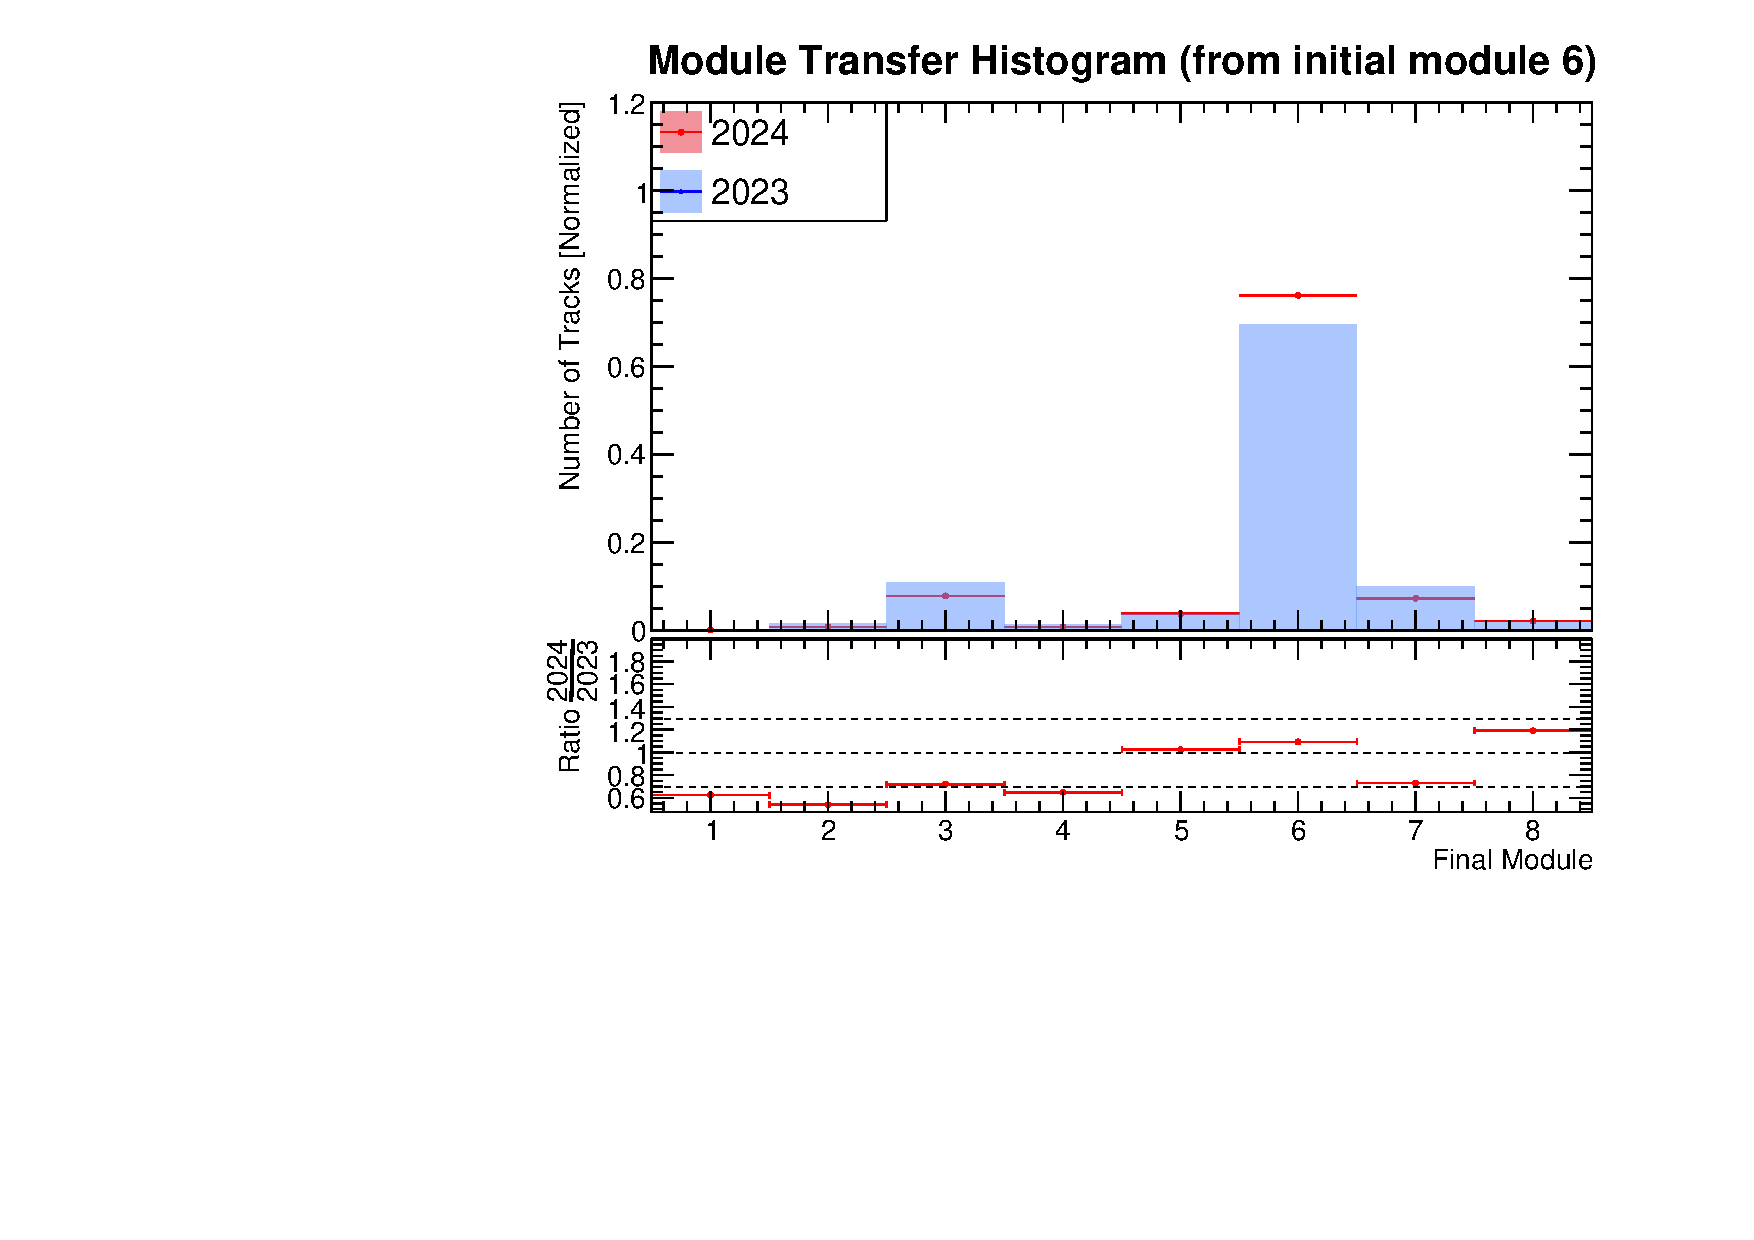
\includegraphics[width=\linewidth]{./ModuleLevelPlots/final_module_from_st0_module6.pdf}
%         \end{subfigure}

%         \begin{subfigure}[t]{0.49\linewidth}
%             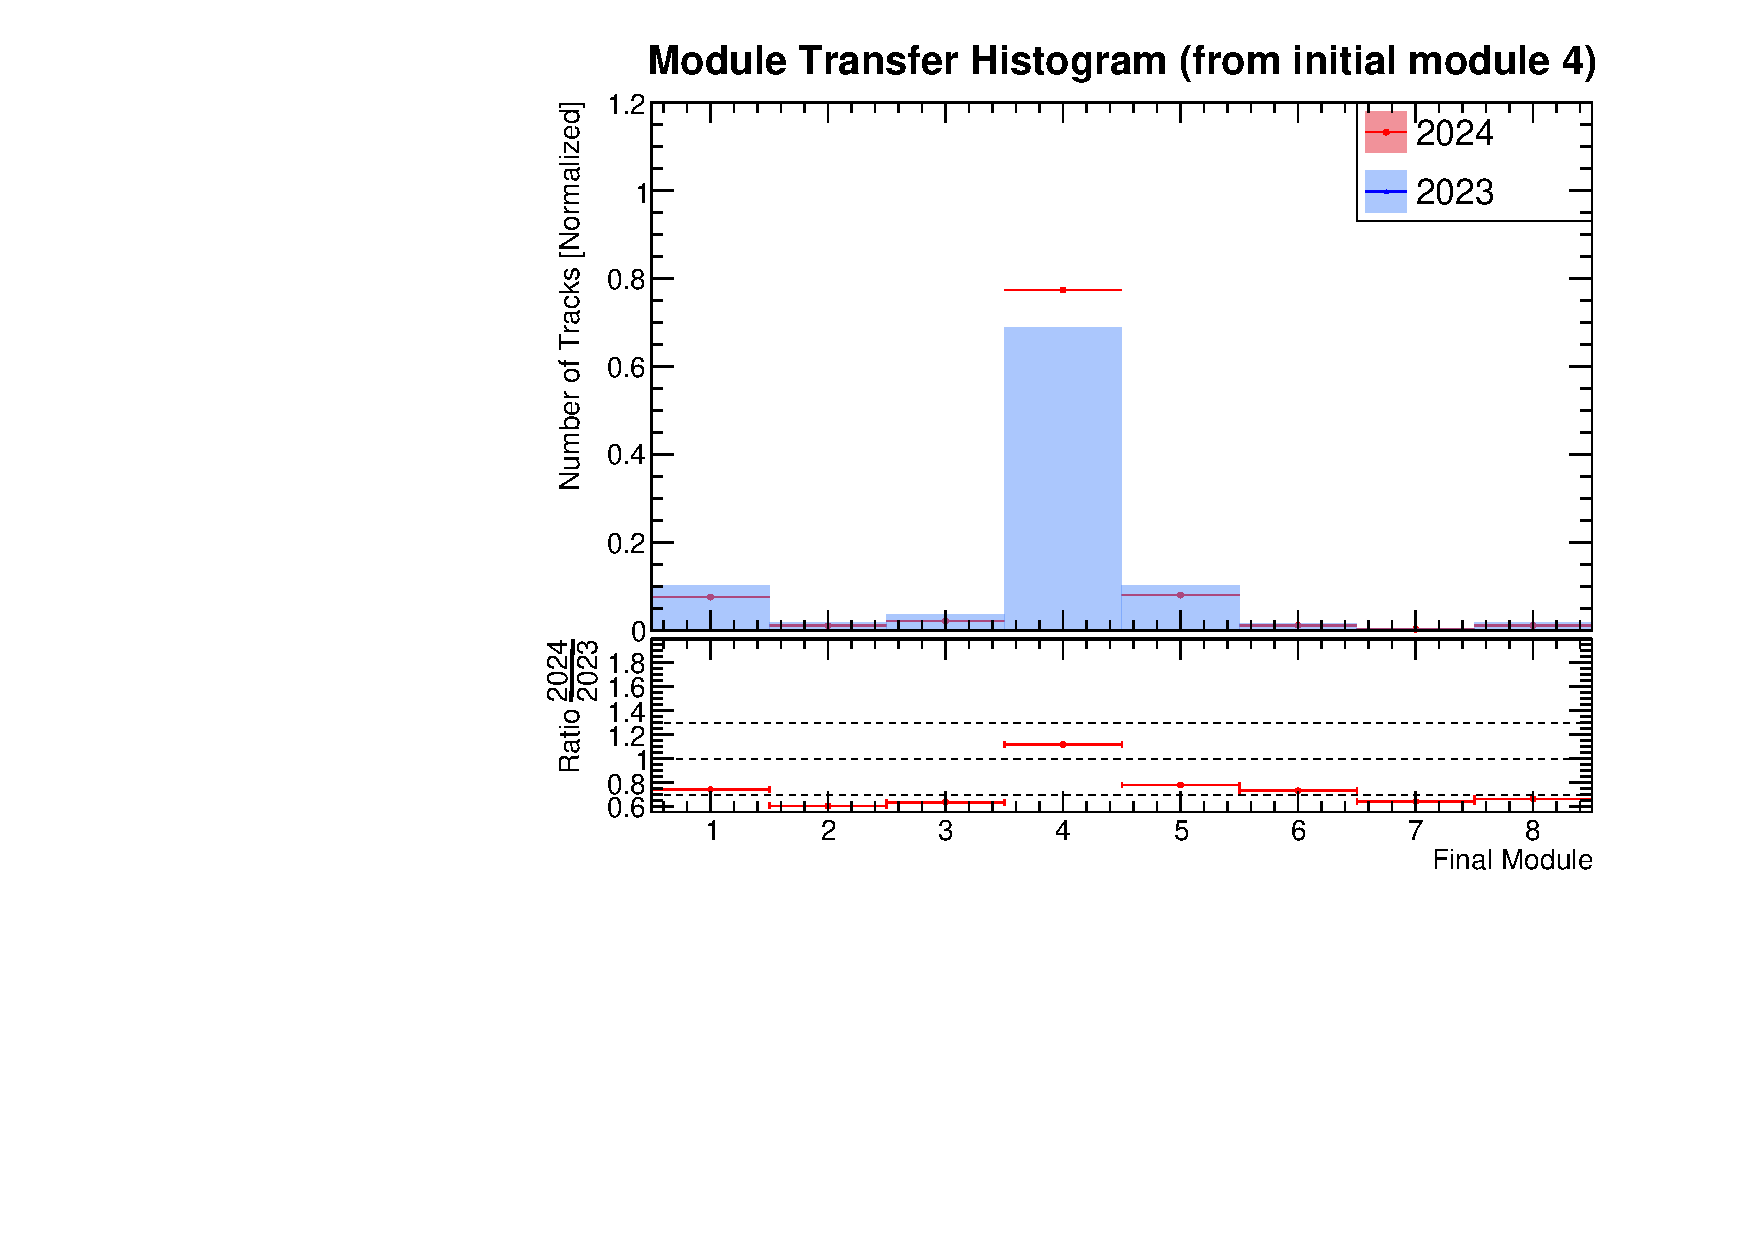
\includegraphics[width=\linewidth]{./ModuleLevelPlots/final_module_from_st0_module4.pdf}
%         \end{subfigure}
%         \begin{subfigure}[t]{0.49\linewidth}
%             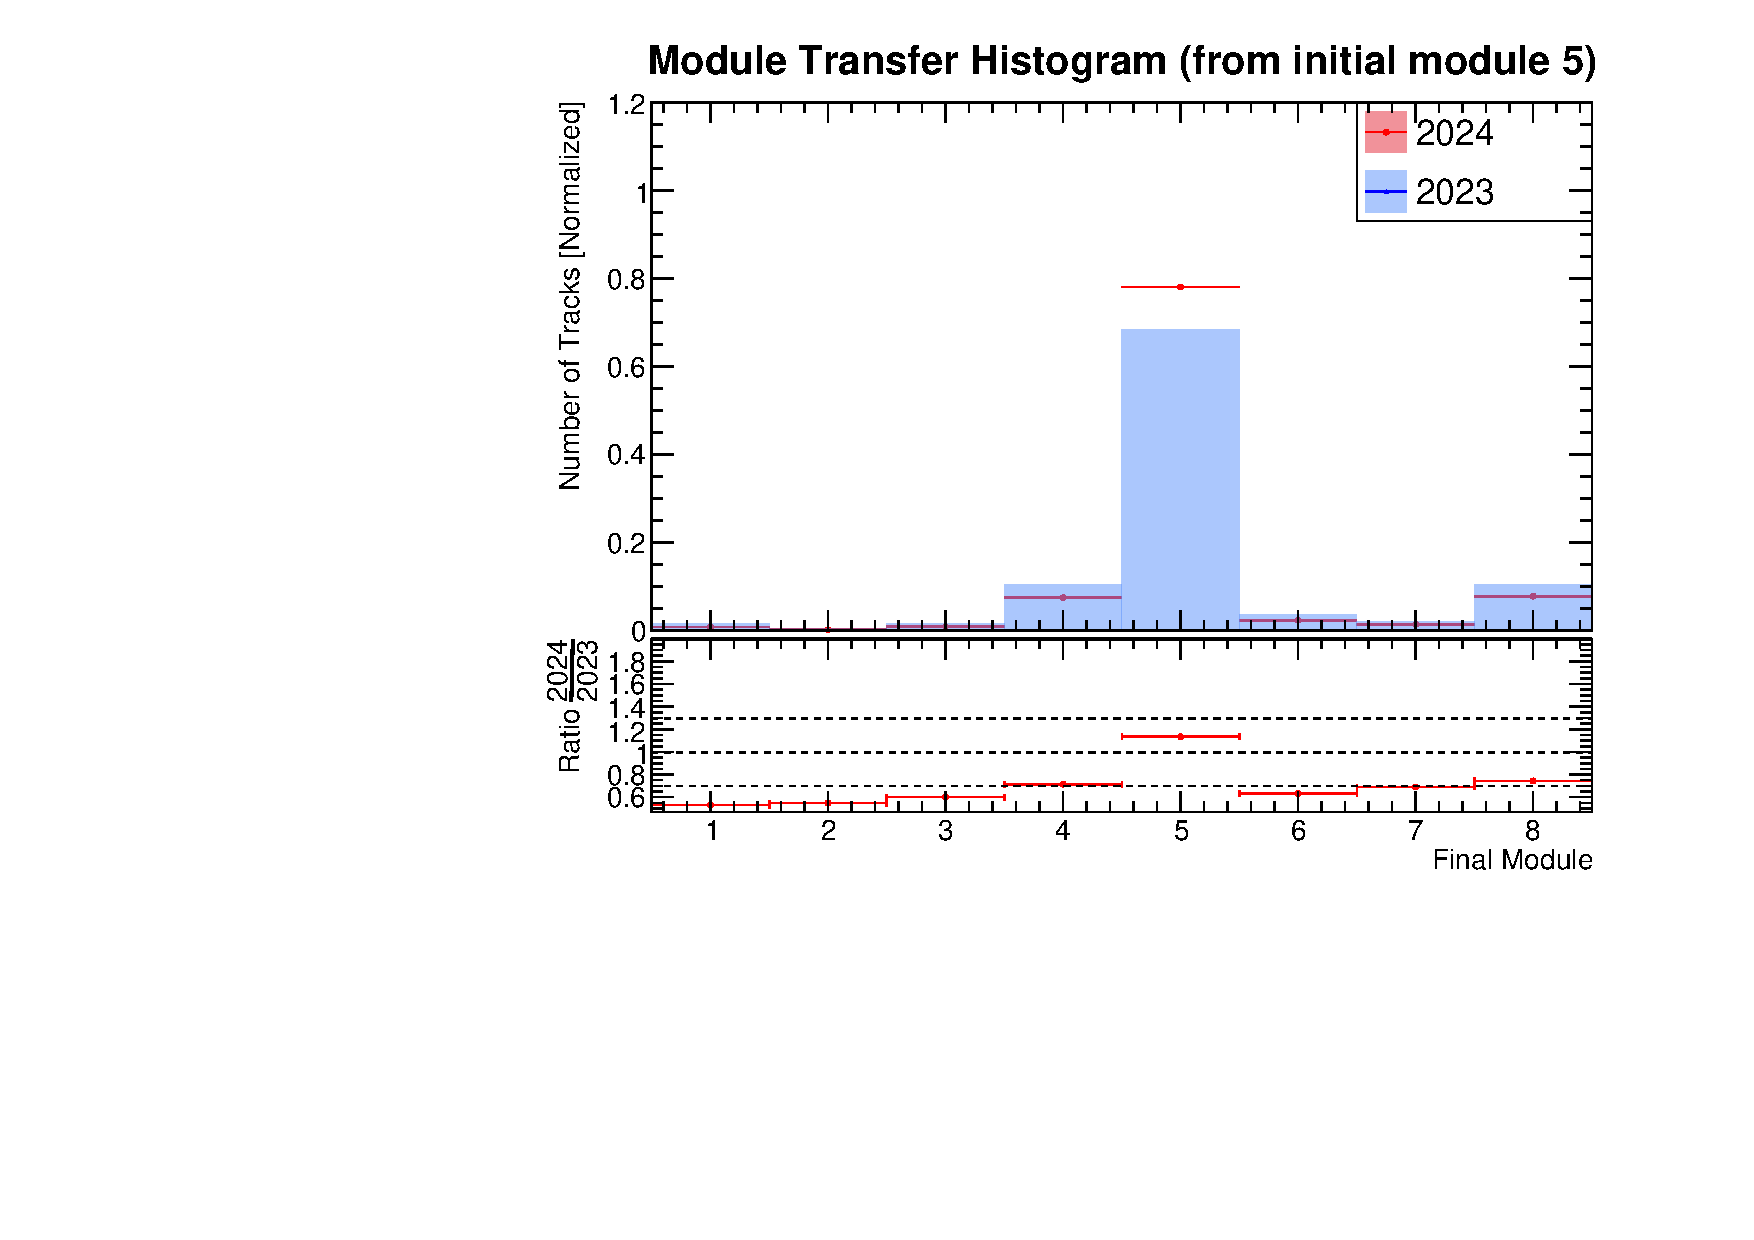
\includegraphics[width=\linewidth]{./ModuleLevelPlots/final_module_from_st0_module5.pdf}
%         \end{subfigure}
%     \end{figure}
% \end{frame}

% \section{Track Parameters Modulewise}    

\begin{frame}{Modulewise Track Parameters}
    
    Recap of the Track Parameters:
    \begin{itemize}
        \item Number of longTracks
        \item Track Charge
        \item Track Chi2 
        \item Track nDoF
        \item TracK Momenta 
        \item Track Chi2perDoF [SKIP]
        \item Track In Station [SKIP]
        \item Track nLayers [SKIP]
        \item Track Propagation Error [SKIP]
    \end{itemize}
    \vspace{0.3 cm}
    \small{    
    Note: Unfortunately, 8 modules across 2 year = 16 Histograms \\
    An year wise for each module would be too long.
    So we do a module level comparison, year wise plots available in the backup.
    }
    % \begin{itemize}
    %     \item Hard to visualize, so we do a module level comparison
    %     \item More detailed plots available in the backup/repo
    % \end{itemize}
\end{frame}




\newcommand{\makemodulewiseframes}[2]{
    \begin{frame}{#2}
        \newcommand{\colname}{#1}
        \begin{figure}
            \centering
            \begin{subfigure}[t]{0.49\linewidth}
                \includegraphics[width=\linewidth]{./ModuleLevelPlots/\colname_st0_module1.pdf}
            \end{subfigure}
            \begin{subfigure}[t]{0.49\linewidth}
                \includegraphics[width=\linewidth]{./ModuleLevelPlots/\colname_st0_module8.pdf}
            \end{subfigure}
    
            \begin{subfigure}[t]{0.49\linewidth}
                \includegraphics[width=\linewidth]{./ModuleLevelPlots/\colname_st0_module2.pdf}
            \end{subfigure}
            \begin{subfigure}[t]{0.49\linewidth}
                \includegraphics[width=\linewidth]{./ModuleLevelPlots/\colname_st0_module7.pdf}
            \end{subfigure}
        \end{figure}
    \end{frame}
    \begin{frame}{#2 [Contd.]}
        \newcommand{\colname}{#1}
        \begin{figure}
            \centering
            \begin{subfigure}[t]{0.49\linewidth}
                \includegraphics[width=\linewidth]{./ModuleLevelPlots/\colname_st0_module3.pdf}
            \end{subfigure}
            \begin{subfigure}[t]{0.49\linewidth}
                \includegraphics[width=\linewidth]{./ModuleLevelPlots/\colname_st0_module6.pdf}
            \end{subfigure}
    
            \begin{subfigure}[t]{0.49\linewidth}
                \includegraphics[width=\linewidth]{./ModuleLevelPlots/\colname_st0_module4.pdf}
            \end{subfigure}
            \begin{subfigure}[t]{0.49\linewidth}
                \includegraphics[width=\linewidth]{./ModuleLevelPlots/\colname_st0_module5.pdf}
            \end{subfigure}
        \end{figure}
    \end{frame}

}



% \makemodulewiseframes{longTracks}{Distribution longTracks Modulewise}
\begin{frame}{Distribution longTracks Modulewise}
    \newcommand{\colname}{longTracks}
    \begin{columns}
        \begin{column}{0.6\linewidth}
            \begin{figure}
                \centering
                \includegraphics[width=\linewidth]{./ModuleLevelPlots/\colname_st0_2023.pdf}
            \end{figure}
        \end{column}
        \begin{column}{0.6\linewidth}
            \begin{figure}
                \centering
                \includegraphics[width=\linewidth]{./ModuleLevelPlots/\colname_st0_2024.pdf}
            \end{figure}
        \end{column}
    \end{columns}
    \begin{itemize}
        \item 2024 has more events in the tail
        \item Seem to form two groups with [for other Parameters as well]
        \begin{itemize}
            \item Modules 2,7,8 having lower long tracks [pronounced in bin2]
            \item Separation between groups worse with higher longTracks
        \end{itemize}
    \end{itemize}
\end{frame}

% \makemodulewiseframes{Track_charge}{Distribution of Track Charge Modulewise}
\begin{frame}{Distribution Track Charge Modulewise}
    \newcommand{\colname}{Track_charge}
    \begin{columns}
        \begin{column}{0.6\linewidth}
            \begin{figure}
                \centering
                \includegraphics[width=\linewidth]{./ModuleLevelPlots/\colname_st0_2023.pdf}
            \end{figure}
        \end{column}
        \begin{column}{0.6\linewidth}
            \begin{figure}
                \centering
                \includegraphics[width=\linewidth]{./ModuleLevelPlots/\colname_st0_2024.pdf}
            \end{figure}
        \end{column}
    \end{columns}

    \begin{itemize}
        \small
        \item 2023 has more negatively charged tracks
        \item In 2023 Module 1,2 seem to get more positively charged tracks
        \item In 2024 Module 3,6,7,5 seem to get more positively charged tracks
        \begin{itemize}
            \item Suggests, positive tracks concentrated in the bottom right?
        \end{itemize}
    \end{itemize}
\end{frame}

% \makemodulewiseframes{Track_Chi2}{Track Chi2 Modulewise}
\begin{frame}{Track Chi2 Modulewise}
    \newcommand{\colname}{Track_Chi2}
    \begin{columns}
        \begin{column}{0.6\linewidth}
            \begin{figure}
                \centering
                \includegraphics[width=\linewidth]{./ModuleLevelPlots/\colname_st0_2023.pdf}
            \end{figure}
        \end{column}
        \begin{column}{0.6\linewidth}
            \begin{figure}
                \centering
                \includegraphics[width=\linewidth]{./ModuleLevelPlots/\colname_st0_2024.pdf}
            \end{figure}
        \end{column}
    \end{columns}

    \begin{itemize}
        \small
        \item Better Agreement in 2024 amongst modules
        \item Module 2 shows higher Track Chi2 in 2023
    \end{itemize}
\end{frame}

% \makemodulewiseframes{Track_nDoF}{Track Degrees of Freedom Modulewise}
\begin{frame}{Track Degrees of Freedom Modulewise}
    \newcommand{\colname}{Track_nDoF}
    \begin{columns}
        \begin{column}{0.6\linewidth}
            \begin{figure}
                \centering
                \includegraphics[width=\linewidth]{./ModuleLevelPlots/\colname_st0_2023.pdf}
            \end{figure}
        \end{column}
        \begin{column}{0.6\linewidth}
            \begin{figure}
                \centering
                \includegraphics[width=\linewidth]{./ModuleLevelPlots/\colname_st0_2024.pdf}
            \end{figure}
        \end{column}
    \end{columns}

    \begin{itemize}
        \small
        \item Module 2 has significantly higher nDoF in 2024
        \item In 2024 more tracks have nDof $\geq 20$
        \item Track NDoF split into two groups
        \begin{itemize}
            \item Higher nDoF Modules : 2, 1, 8, 7 [Modules with y $\geq$ 0]
            \item Lower nDoF Modules \ : 3, 4, 5, 6  [Modules with y $\leq$ 0]
        \end{itemize}
    \end{itemize}
\end{frame}

% \makemodulewiseframes{Track_Chi2perDoF}{Track Chi2perDoF Modulewise}
% \begin{frame}{Track Chi2perDoF Modulewise}
%     \newcommand{\colname}{Track_Chi2perDoF}
%     \begin{columns}
%         \begin{column}{0.6\linewidth}
%             \begin{figure}
%                 \centering
%                 \includegraphics[width=\linewidth]{./ModuleLevelPlots/\colname_st0_2023.pdf}
%             \end{figure}
%         \end{column}
%         \begin{column}{0.6\linewidth}
%             \begin{figure}
%                 \centering
%                 \includegraphics[width=\linewidth]{./ModuleLevelPlots/\colname_st0_2024.pdf}
%             \end{figure}
%         \end{column}
%     \end{columns}

%     \begin{itemize}
%         \small
%         \item In 2023, the Track Chi2 seem to split into two groups
%         \begin{itemize}
%             \item Higher Chi2 Modules : 2, 1, 8, 7 [Modules with y $\geq$ 0]
%             \item Lower Chi2 Modules \ : 3, 4, 5, 6  [Modules with y $\leq$ 0]
%         \end{itemize}
%     \end{itemize}
% \end{frame}

% \makemodulewiseframes{Track_nLayers}{Distribution of Track\_nLayers Modulewise}
% \begin{frame}{Distribution of Track\_nLayers Modulewise}
%     \newcommand{\colname}{Track_nLayers}
%     \begin{columns}
%         \begin{column}{0.6\linewidth}
%             \begin{figure}
%                 \centering
%                 \includegraphics[width=\linewidth]{./ModuleLevelPlots/\colname_st0_2023.pdf}
%             \end{figure}
%         \end{column}
%         \begin{column}{0.6\linewidth}
%             \begin{figure}
%                 \centering
%                 \includegraphics[width=\linewidth]{./ModuleLevelPlots/\colname_st0_2024.pdf}
%             \end{figure}
%         \end{column}
%     \end{columns}

%     \begin{itemize}
%         \small
%         \item Again seem to split into two groups
%         \begin{itemize}
%             \item Higher nLayer Modules : 2, 1, 8, 7 [Modules with y $\geq$ 0]
%             \item Lower nLayer Modules \ : 3, 4, 5, 6  [Modules with y $\leq$ 0]
%         \end{itemize}
%     \end{itemize}
% \end{frame}

\begin{frame}{Track Momenta Modulewise}
    \begin{figure}
        \centering
        \begin{subfigure}[t]{0.49\linewidth}
            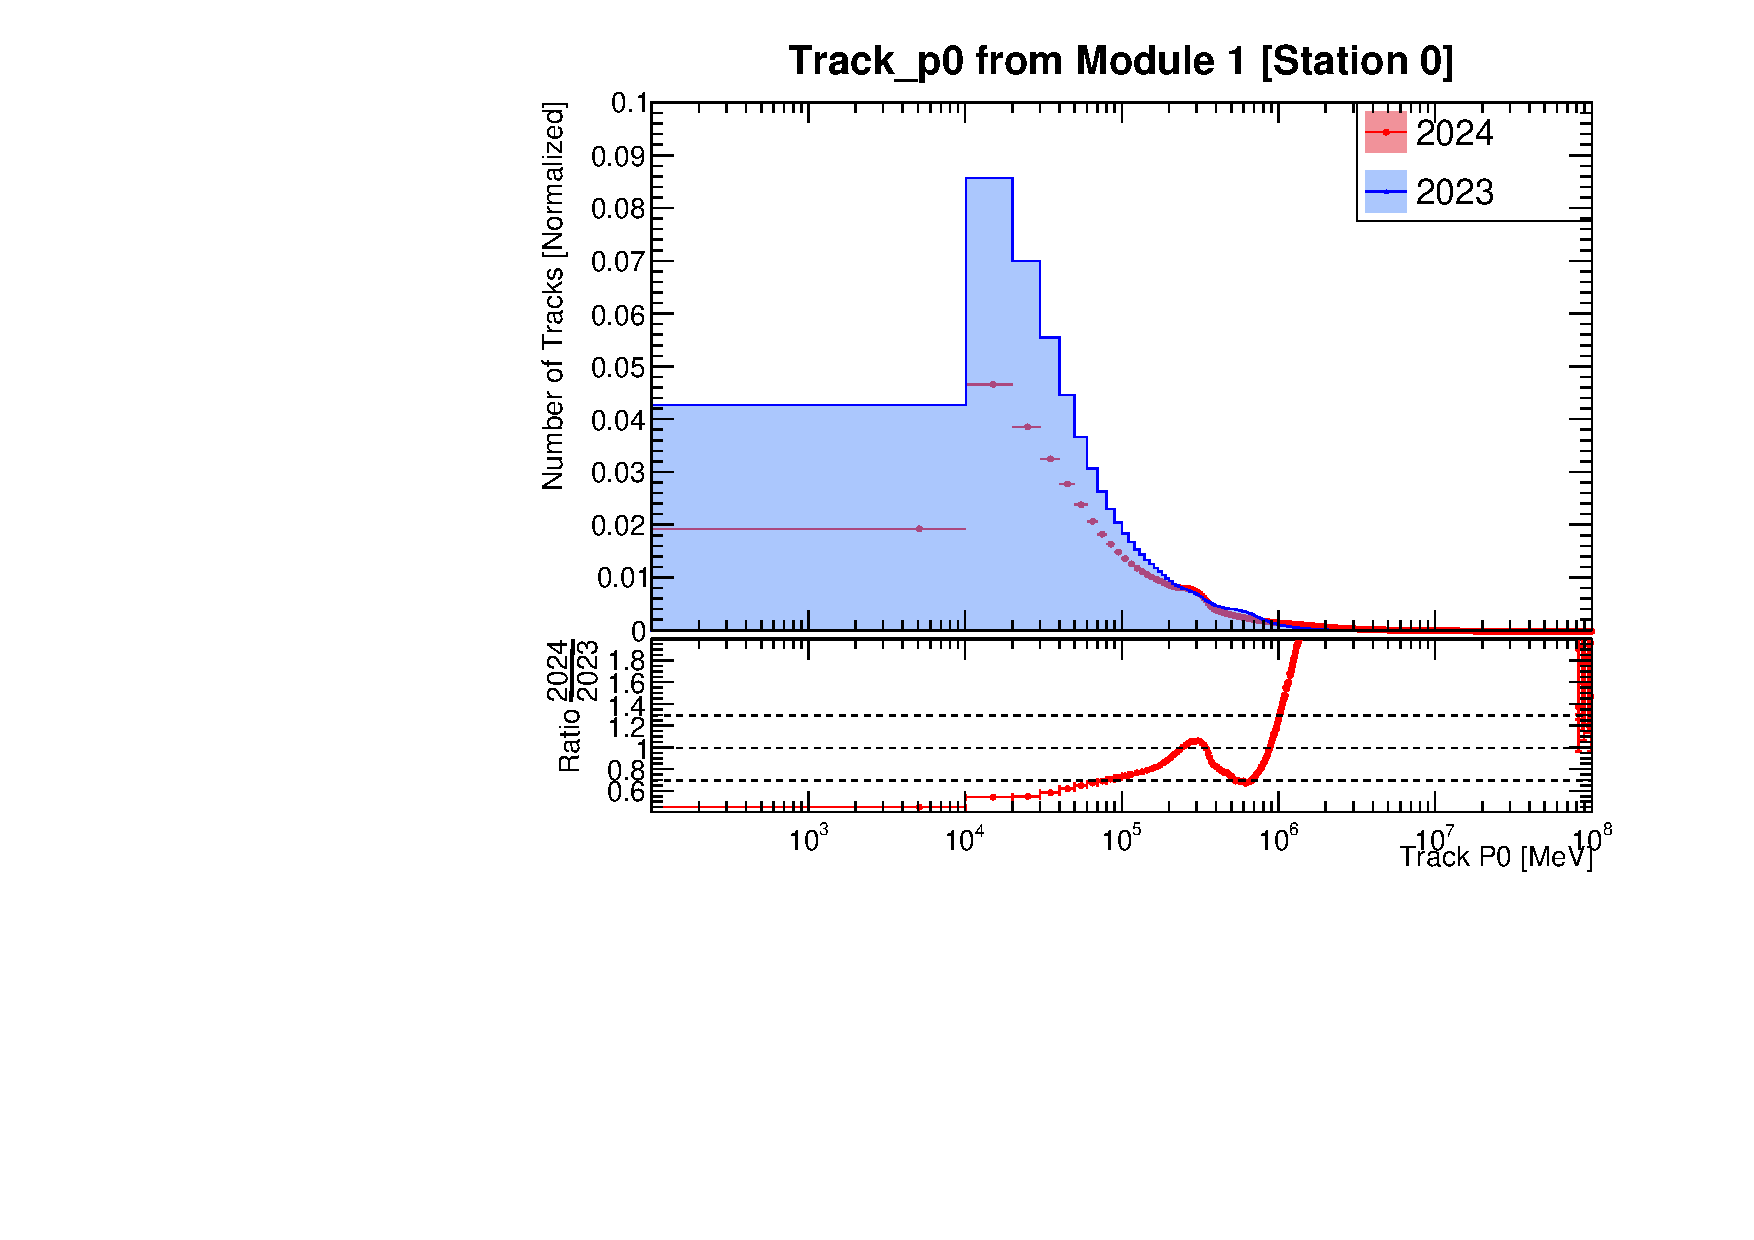
\includegraphics[width=\linewidth]{./ModuleLevelPlots/Track_p0_st0_module1_linear.pdf}
        \end{subfigure}
        \begin{subfigure}[t]{0.49\linewidth}
            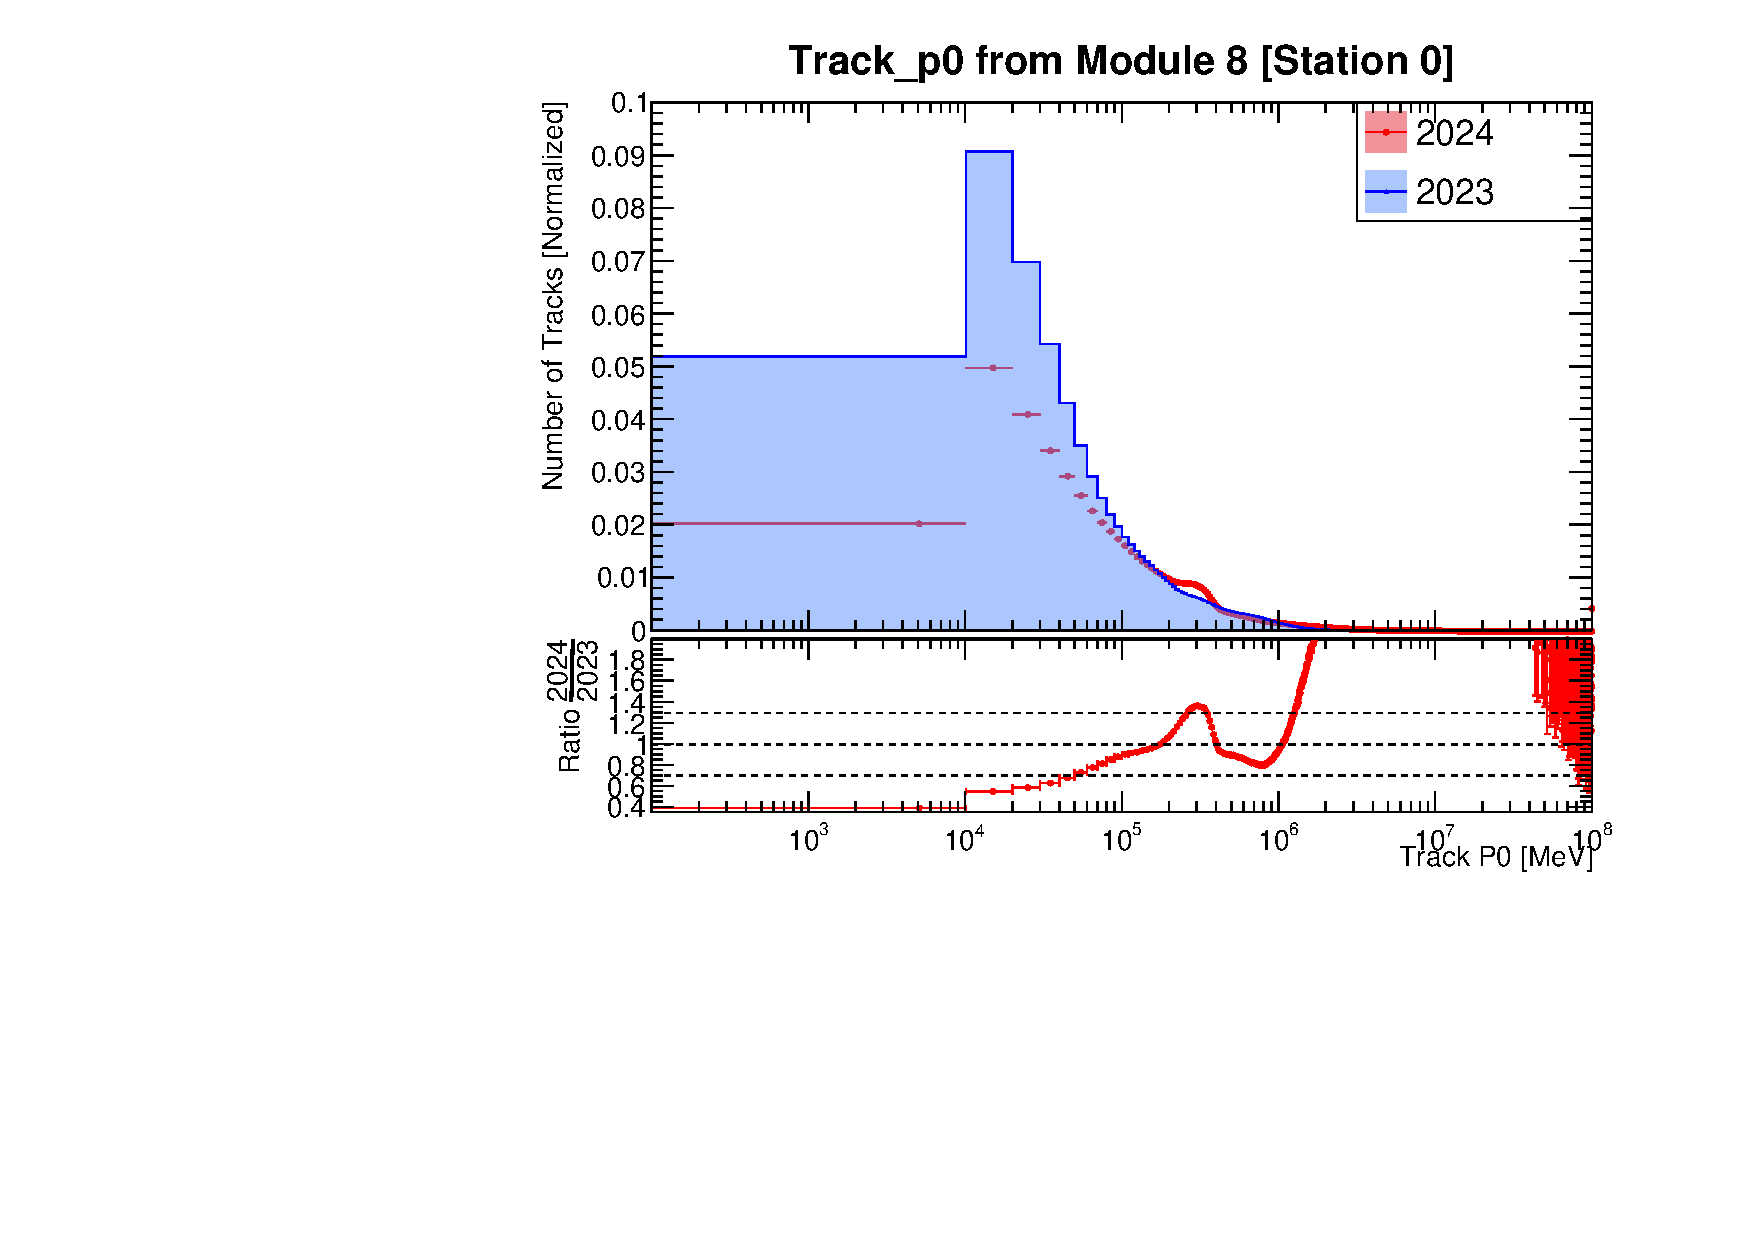
\includegraphics[width=\linewidth]{./ModuleLevelPlots/Track_p0_st0_module8_linear.pdf}
        \end{subfigure}

        \begin{subfigure}[t]{0.49\linewidth}
            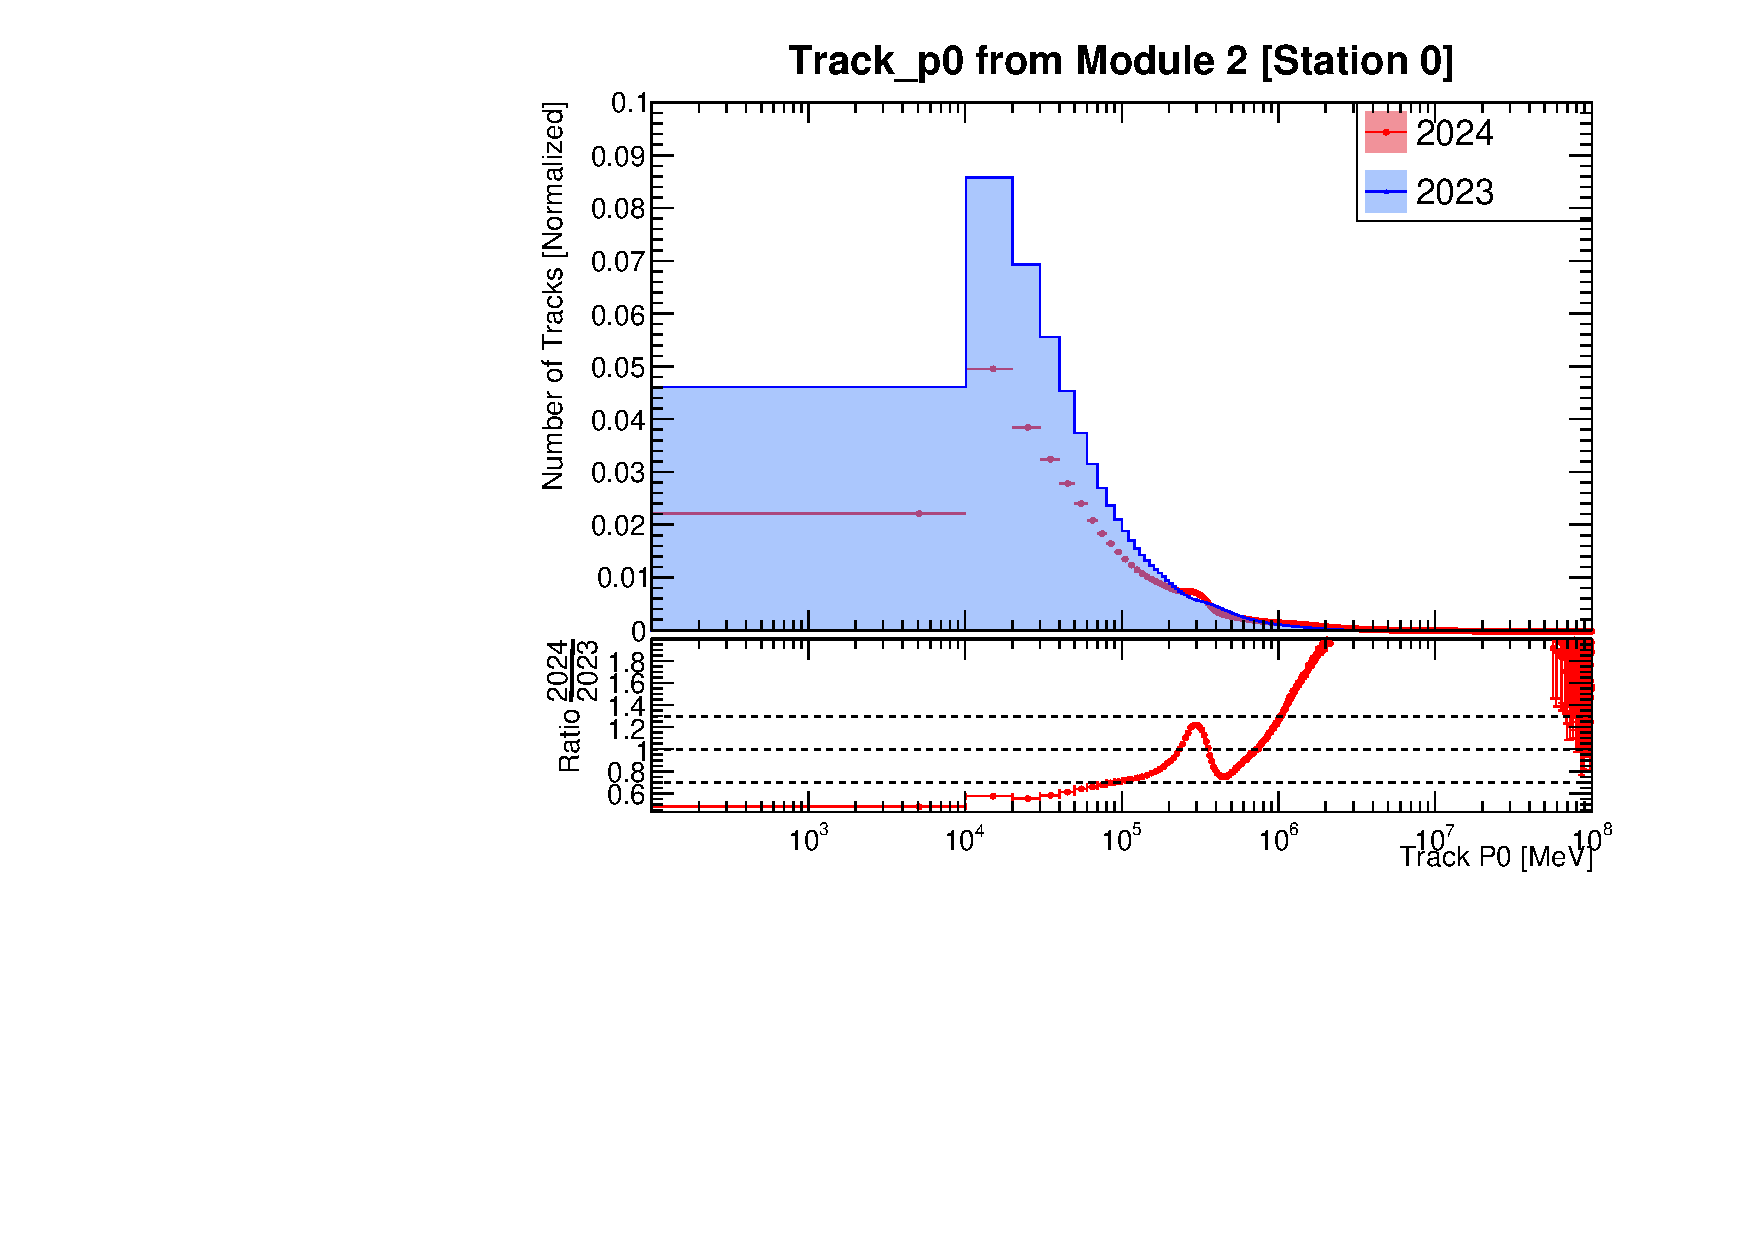
\includegraphics[width=\linewidth]{./ModuleLevelPlots/Track_p0_st0_module2_linear.pdf}
        \end{subfigure}
        \begin{subfigure}[t]{0.49\linewidth}
            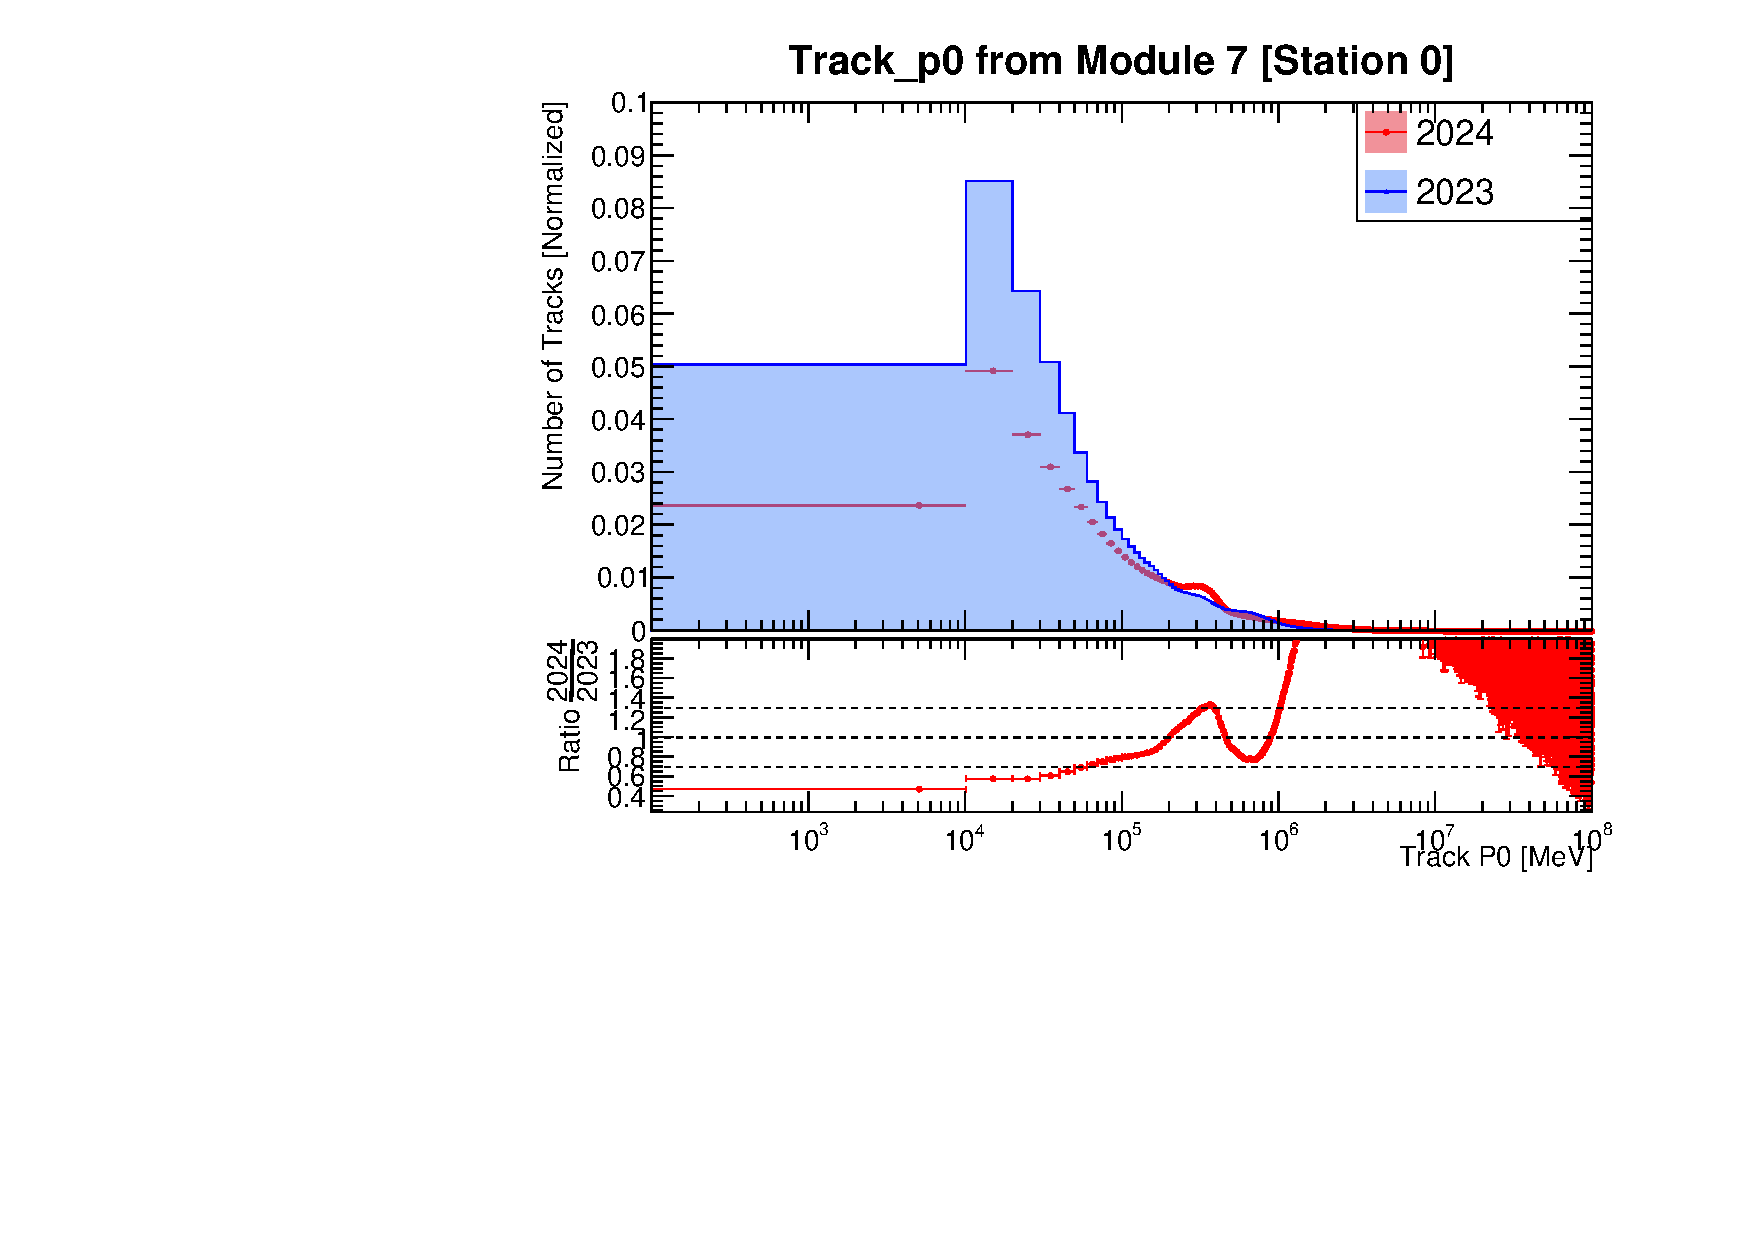
\includegraphics[width=\linewidth]{./ModuleLevelPlots/Track_p0_st0_module7_linear.pdf}
        \end{subfigure}
    \end{figure}
\end{frame}

\begin{frame}{Track Momenta Modulewise [Contd.]}
    \begin{figure}
        \centering
        \begin{subfigure}[t]{0.49\linewidth}
            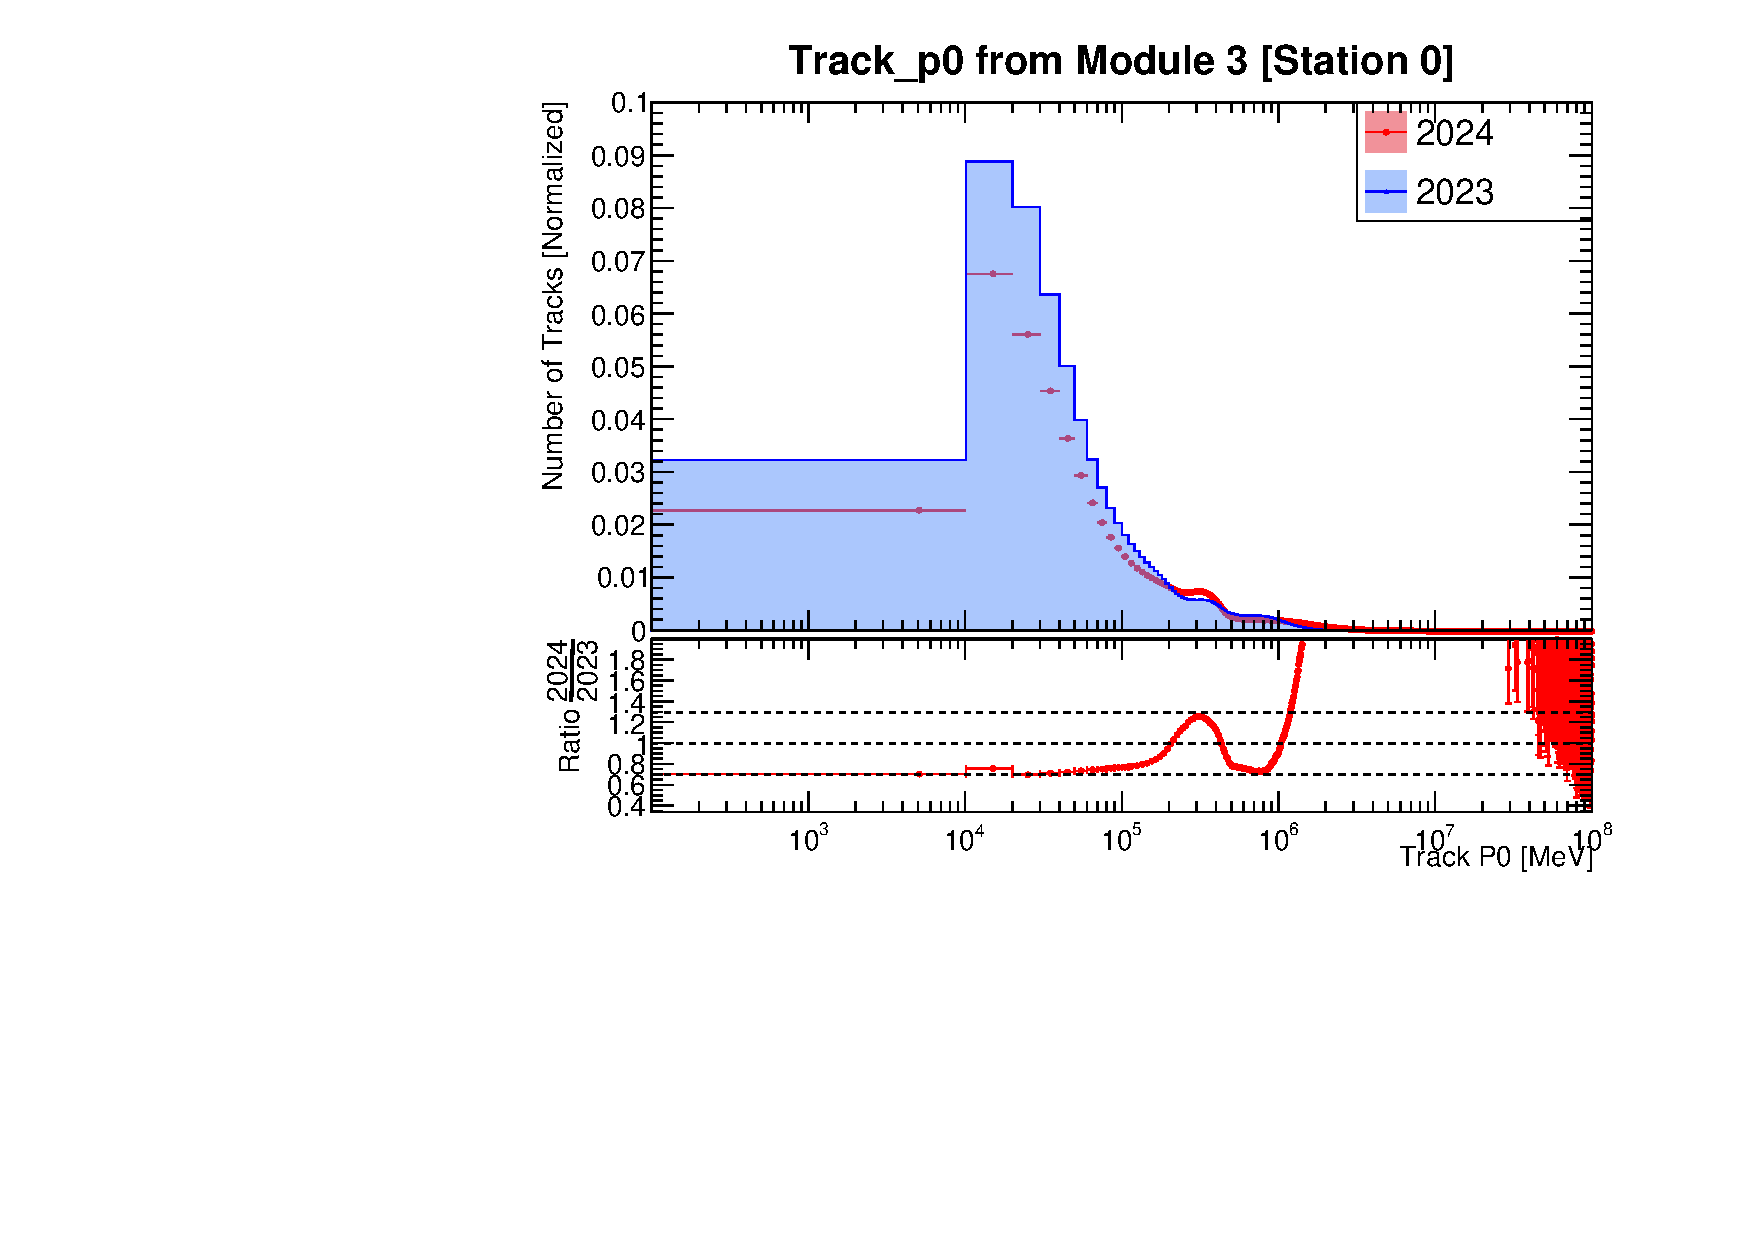
\includegraphics[width=\linewidth]{./ModuleLevelPlots/Track_p0_st0_module3_linear.pdf}
        \end{subfigure}
        \begin{subfigure}[t]{0.49\linewidth}
            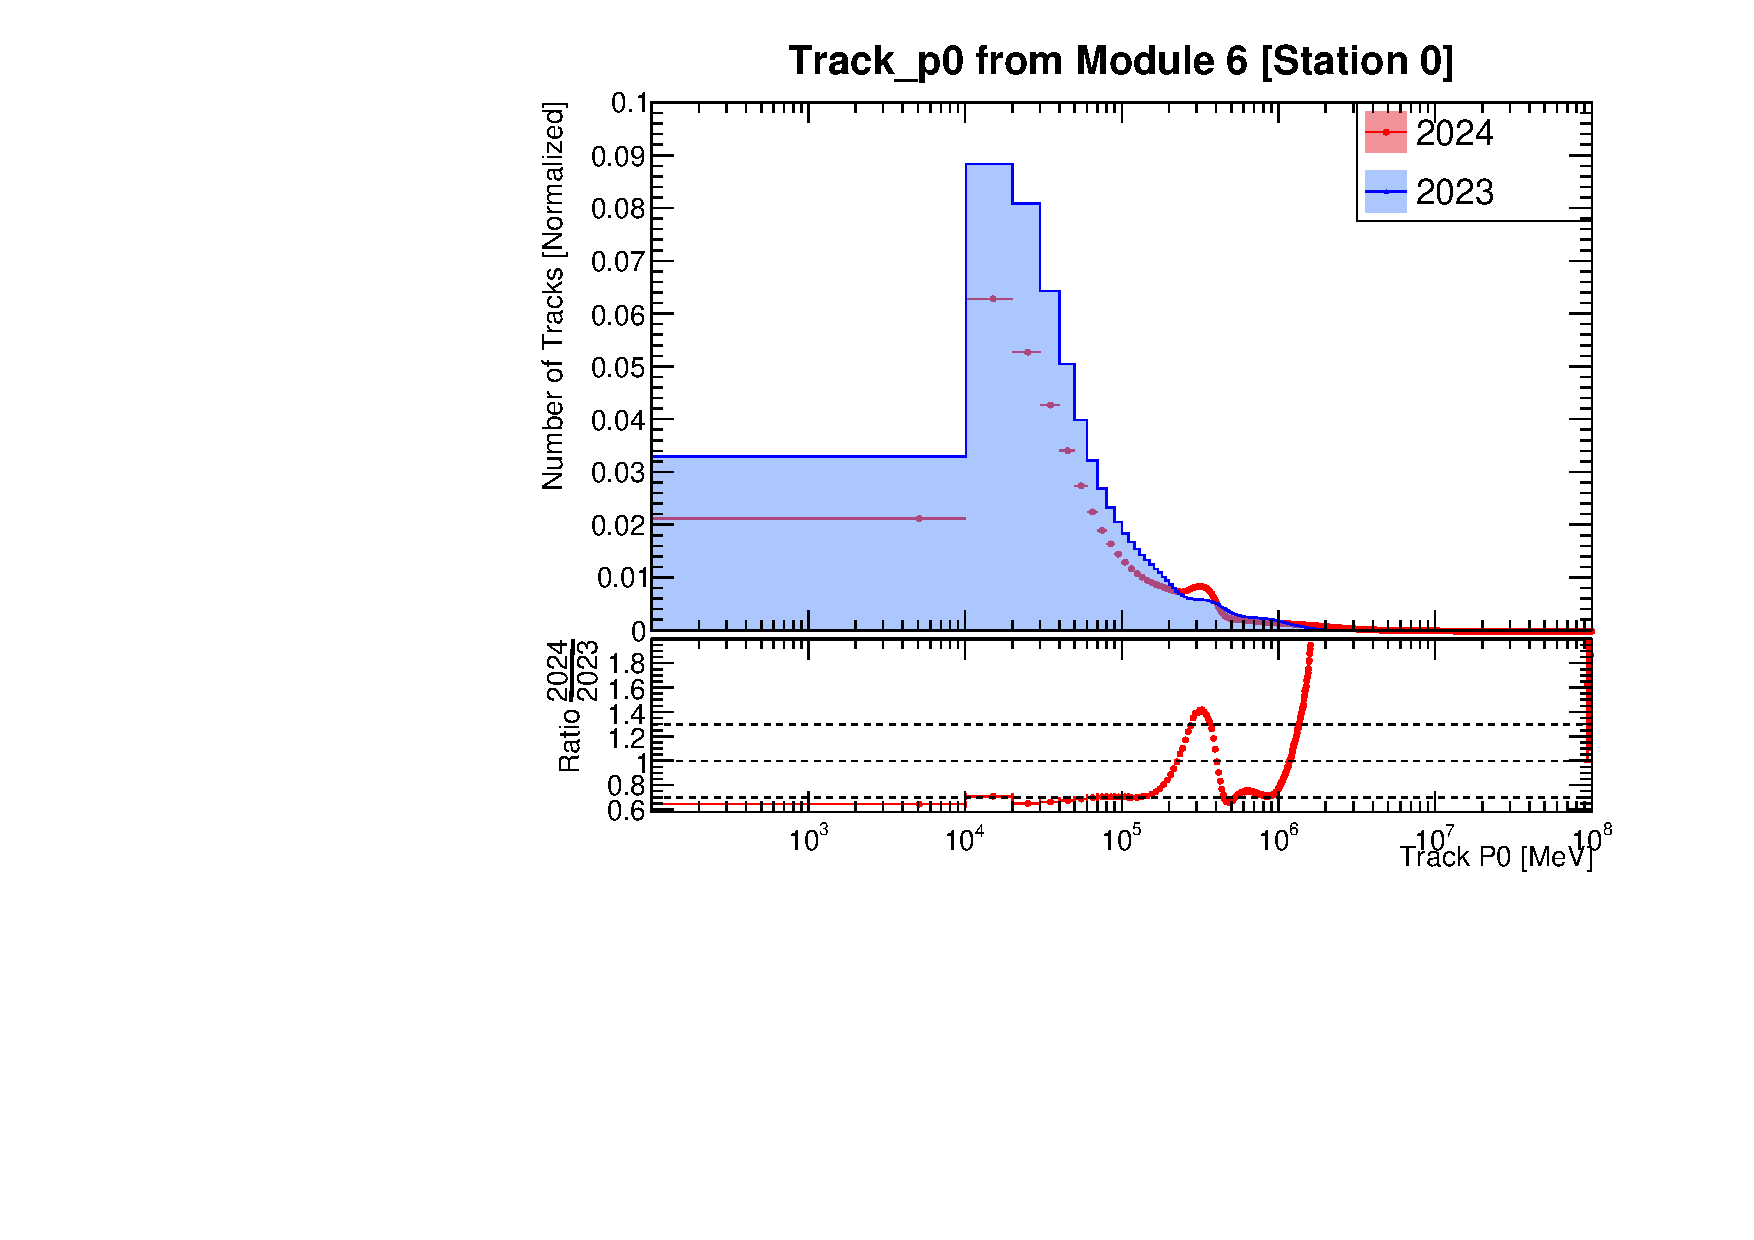
\includegraphics[width=\linewidth]{./ModuleLevelPlots/Track_p0_st0_module6_linear.pdf}
        \end{subfigure}

        \begin{subfigure}[t]{0.49\linewidth}
            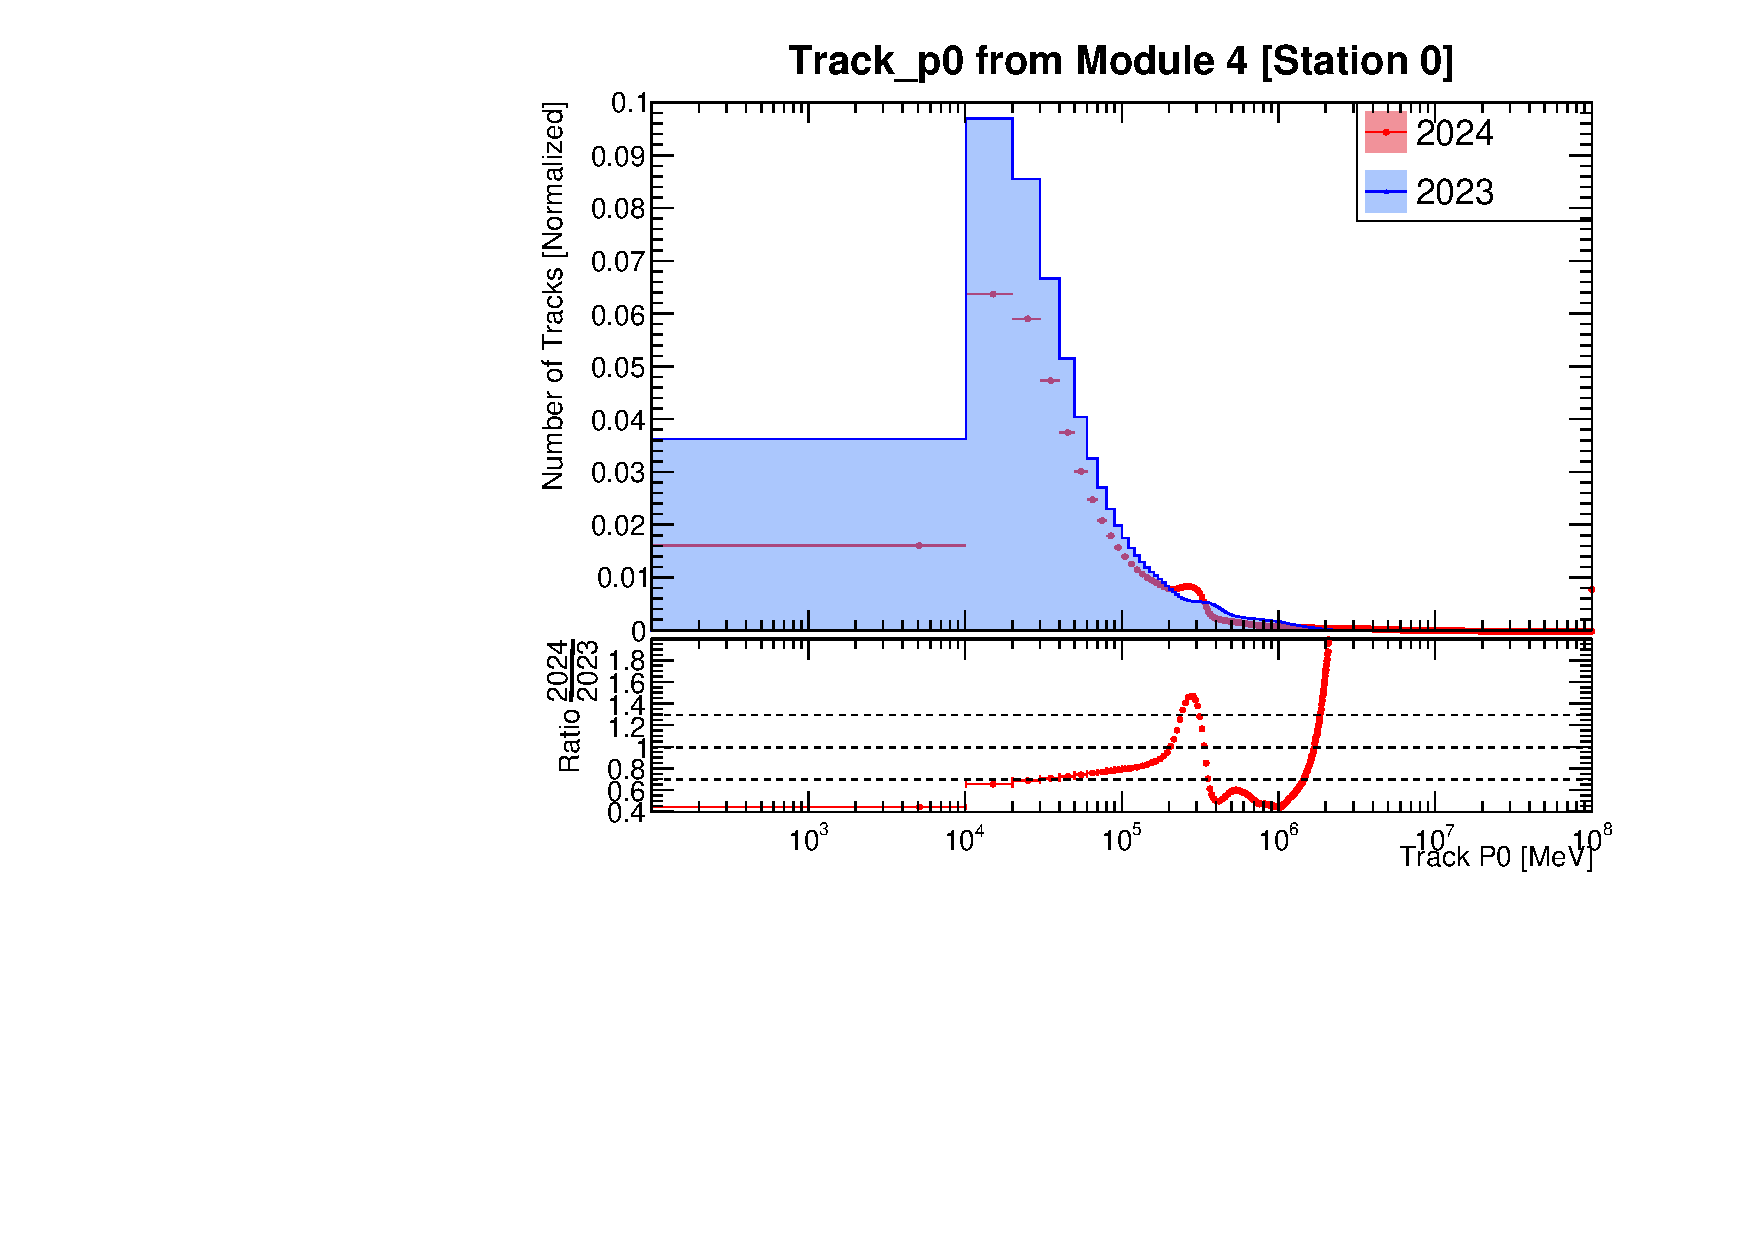
\includegraphics[width=\linewidth]{./ModuleLevelPlots/Track_p0_st0_module4_linear.pdf}
        \end{subfigure}
        \begin{subfigure}[t]{0.49\linewidth}
            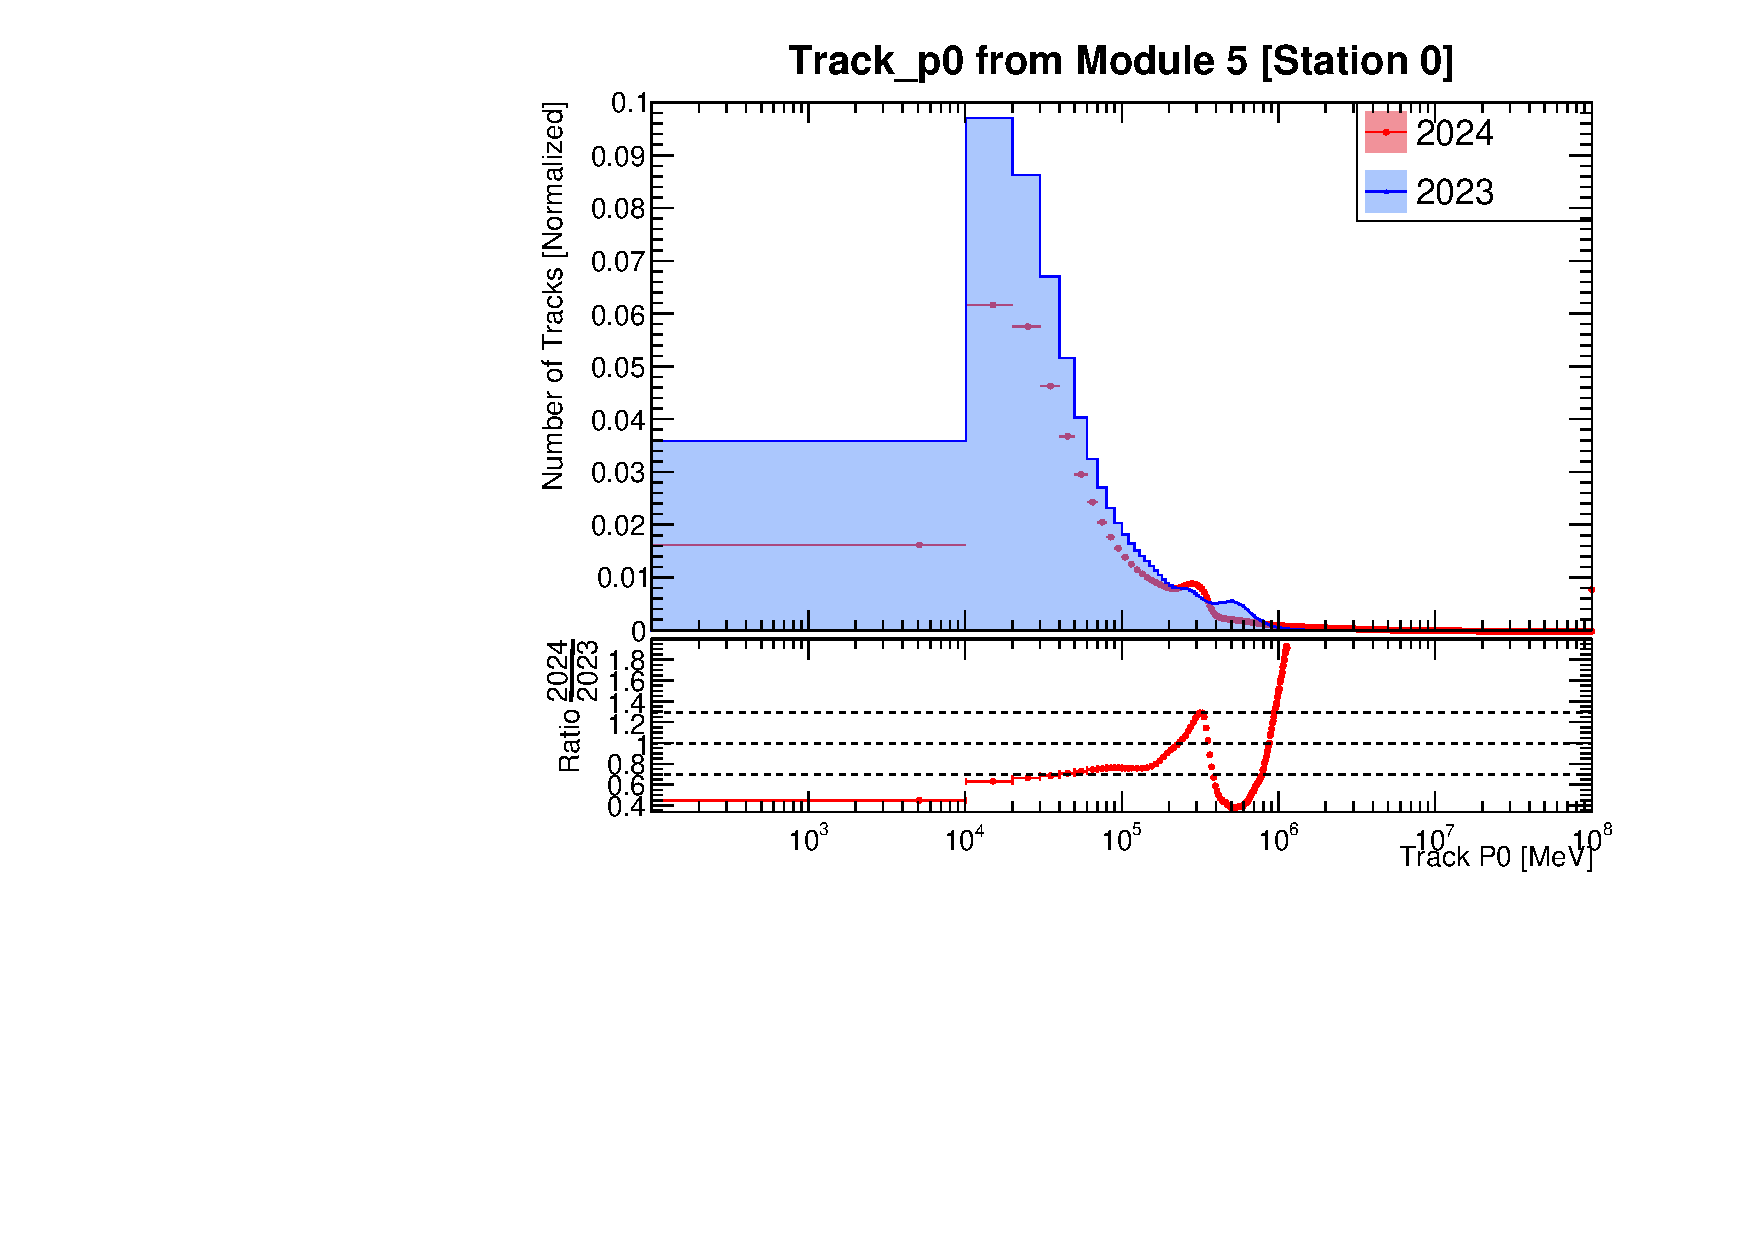
\includegraphics[width=\linewidth]{./ModuleLevelPlots/Track_p0_st0_module5_linear.pdf}
        \end{subfigure}
    \end{figure}
\end{frame}

\begin{frame}{Distribution of Track Momenta Modulewise}
    \begin{columns}
        \begin{column}{0.6\linewidth}
            \begin{figure}
                \centering
                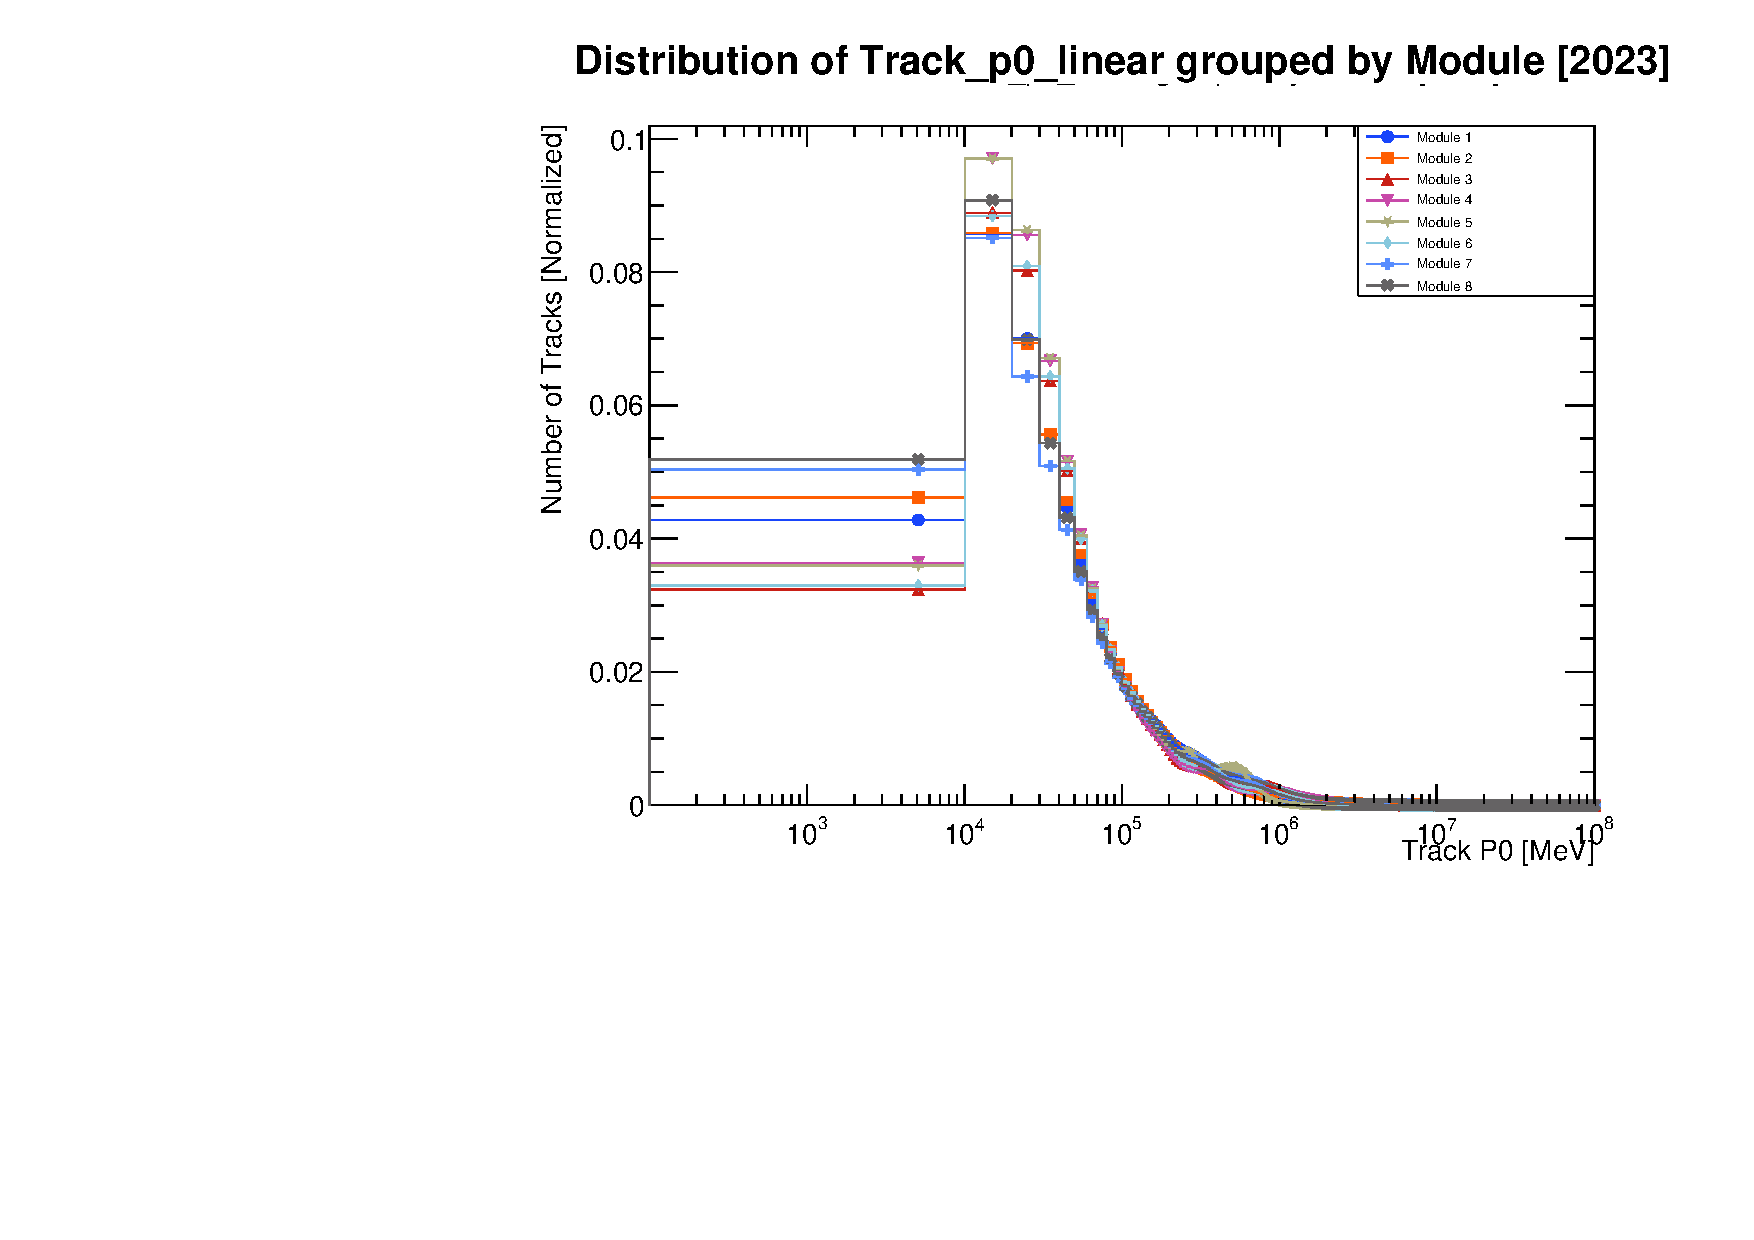
\includegraphics[width=\linewidth]{./ModuleLevelPlots/Track_p0_linear_st0_2023.pdf}
            \end{figure}
        \end{column}
        \begin{column}{0.6\linewidth}
            \begin{figure}
                \centering
                \includegraphics[width=\linewidth]{./ModuleLevelPlots/Track_p0_linear_st0_2024.pdf}
            \end{figure}
        \end{column}
    \end{columns}

    \begin{itemize}
        \small
        \item Again seem to split into two groups in 2024
        \begin{itemize}
            \item Higher Momenta Modules : 3, 4, 5, 6  [Modules with y $\leq$ 0]
            \item Lower Momenta Modules \ : 2, 1, 8, 7 [Modules with y $\geq$ 0]
        \end{itemize}
    \end{itemize}
\end{frame}

% \begin{frame}{Summary of Module Level Analysis}
    
% \end{frame}